\documentclass[fontsize=11pt,%
twoside,% oneside als Alternative m\"{o}glich
BCOR          = 8mm, % bei Bedarf anzupassen
DIV           = 11,  % kann nach Belieben geändert werden
titlepage     = off,%
index=totoc,%
xcolor        = pdftex,%
dvipsnames,%
bibliography  = totoc,%
bibliography = numbered, % bei Bedarf einschalten
listof        = notnumbered]{scrreprt}

\usepackage[left=3.5cm,right=2cm,top=2.5cm,bottom=2cm]{geometry}
\usepackage[english]{babel}                         %deutsches Sprachpacket
\usepackage[utf8]{inputenc}                         %input utf8
\usepackage[official]{eurosym}                      %Symbolsatz
\usepackage{amsmath}                                %Mathepacket
\usepackage{siunitx}                                %Package für zwei nachfolgende Befehle
\sisetup{locale=UK}
\sisetup{per-mode=fraction}
\usepackage{graphicx}                               %Bilder einfügen
\usepackage{subfigure}                              %Subfigures erstellen
\usepackage{subcaption}
\usepackage[onehalfspacing]{setspace}               %für Abstände
\usepackage{booktabs}                               %Für Ruler in Tabellen
\usepackage{makecell}
\usepackage{caption}
\usepackage{tabulary}
\usepackage{tabularx}
\usepackage{array}
\usepackage[table]{xcolor}
\definecolor{light grey}{RGB}{182,182,182}
\usepackage{rotating}
\usepackage{tablefootnote}
\usepackage{refcount}
\usepackage{hhline}
\usepackage{adjustbox}
\usepackage{subcaption}
\usepackage{float}
\usepackage{acronym}
\usepackage{listings}
\definecolor{codegreen}{rgb}{0,0.6,0}
\definecolor{codegrey}{rgb}{0.5,0.5,0.5}
\definecolor{codepurple}{rgb}{0.58,0,0.82}
\definecolor{backcolour}{rgb}{0.95,0.95,0.92}
\definecolor{codeblue}{rgb}{0.0,0.4,0.8}
\lstset{
	language=C++,                       % Sprache auf C++ setzen
	backgroundcolor=\color{backcolour}, % Hintergrundfarbe
	commentstyle=\color{codegreen},    % Farbe für Kommentare (z.B. // )
	keywordstyle=\color{codeblue}\bfseries, % Farbe für Keywords (int, auto, void, ...)
	numberstyle=\tiny\color{codegrey},  % Stil der Zeilennummern
	stringstyle=\color{codepurple},     % Farbe für Strings ("Text")
	basicstyle=\ttfamily\small,         % Festbreitenschriftart für den Code
	breakatwhitespace=false,            
	breaklines=true,                    % Automatische Zeilenumbrüche bei langen Zeilen
	captionpos=b,                       % Beschriftung unter dem Codeblock
	keepspaces=true,                    
	numbers=left,                       % Zeilennummern links anzeigen
	numbersep=5pt,                      % Abstand der Nummern zum Code
	showspaces=false,                
	showstringspaces=false,
	showtabs=false,                  
	tabsize=4,                          % Tabulatorbreite
	frame=single,                       % Rahmen um den Codeblock
	rulecolor=\color{gray!30}           % Farbe des Rahmens
}
\usepackage{accents}
\usepackage[stable]{footmisc}
\usepackage{pdfpages}
\usepackage[
backend=biber,
style=numeric,
sorting=none
]{biblatex}
\DefineBibliographyStrings{english}{
	bibliography = {References}
}
\addbibresource{mybibFile.bib} %Import the bibliography file
\counterwithin{figure}{section}
\counterwithin{table}{section}
\counterwithin{equation}{section}

\begin{document}

\begin{titlepage}
	\centering

	\begin{center}
	\captionsetup{font=footnotesize}
	\begin{figure}[!h]
		\subfigure{
\includegraphics[height=1.75cm]{THM-logo-eps-converted-to.pdf}}
        \hspace{0.5cm}
		\subfigure{
\includegraphics[height=2.5cm]{sprog-logo-discord.png}}
    \end{figure}
    \end{center}


	{\scshape\LARGE Technische Hochschule Mittelhessen \\ und \\ Spacelfight Rocketry Gießen e.V.\par}
	\vspace{1cm}
	{\scshape\Large Projektarbeit\par}
	\vspace{1cm}
	{\huge\bfseries Development of the Electronic Actuaion \& Guidance for Landing and Elevation (EAGLE) system\par}
	\vspace{0.25cm}
    \rule{\textwidth}{.5pt}
    \vspace{.25cm}
    {\large\bfseries Entwicklung des Electronic Acutation \& Guidance for Landing and Elevation (EAGLE) Systems\par}
    \vspace{.3cm}
	{\Large\scshape SoSe 2025\par}
	\vspace{1cm}
	{\Large \textbf{vorgelegt von}\\ Jason Gläser\par}
	\vfill
	betreut durch\par
    Prof. Dr. Chris Volkmar
	\vfill

% Bottom of the page
	{\large \today\par}
	\cleardoublepage
\end{titlepage}

\setcounter{page}{1}
\pagenumbering{Roman}

\chapter*{Eidesstattliche Erklärung}
Hiermit versichere ich, dass ich die vorliegende Arbeit selbstständig und unter aus
schließlicher Verwendung der angegebenen Literatur und Hilfsmittel erstellt habe. Die
Arbeit wurde bisher in gleicher oder ähnlicher Form keiner anderen Prüfungsbehörde
vorgelegt und nicht veröffentlicht.\\\\

\noindent Ort, Datum: \dotfill \hspace{3mm} Unterschrift: \dotfill 

\newpage


\chapter*{Abstract}
The development of the "Electronic Actuation \& Guidance for Landing and Elevation" (EAGLE) system is a project developed in cooperation with the student rocketry association "Spaceflight Rocketry Gießen e.V." as part of its self-developed on-board computer called "Advances System for Control Electronics, Navigation and Tracking" (ASCENT). Therefore, I would like to thank Spaceflight Rocketry Gießen for giving me the opportunity to pursue the project with their equipment and funding.\\
EAGLE is a avionics module which uses real-time sensor data to accurately estimate the rockets position and attitude as well as detecting mission critical waypoints (such as apogee) to deploy the recovery system, perform the staging and subsequent firing of the sustainer's motor and make real-time decisions about an active aerodynamical airbrake system, which accurately limits the maximum altitude to a preset value.\\
The development process of a printed circuit board for this system according to the rule book provided by the "European Rocketry Challenge" will be the core subject of this project.


\newpage
\tableofcontents
\cleardoublepage

\listoffigures
\cleardoublepage

\listoftables
\cleardoublepage

\chapter*{List of abbreviations}
	\begin{acronym}
		\acro{SRPOG}[SPROG]{\dotfill Spaceflight Rocketry Giessen}
		\acro{eV}[e.V.]{\dotfill eingetragener Verein}
		\acro{EAGLE}[EAGLE]{\dotfill Electronic Acutation \& Guidance for Landing and Eleveation}
		\acro{PIPE}[PIPE]{\dotfill Project for Inital Practical Experimentation}
		\acro{ARCHER}[ARCHER]{\dotfill Aerial Rocket for Competions and High-altitude Experimental Rocketry}
		\acro{PCB}[PCB]{\dotfill Printed Circuit Board}
		\acro{PWM}[PWM]{\dotfill Power Width Modulation}
		\acro{IC}[IC]{\dotfill Integrated circuit}
		\acro{PSU}[PSU]{\dotfill Power supply unit}
		\acro{SMD}[SMD]{\dotfill Surface mounted devices}
		\acro{SPI}[SPI]{\dotfill Serial peripheral interface}
		\acro{I2C}[I2C]{\dotfill Inter-Integrated Circuit}
		\acro{UART}[UART]{\dotfill Universal Asynchronous Receiver-Transmitter}
		\acro{RAM}[RAM]{\dotfill Random access memory}
		\acro{UPDI}[UPDI]{\dotfill Unified Program and Debug Interface}
		\acro{GND}[GND]{\dotfill Ground}
		\acro{ASCENT}[ASCENT]{\dotfill Advanced System for Control Electronics, Navigation and Tracking}
		\acro{EuRoC}[EUROC]{\dotfill European Rocketry Challenge}
		\acro{COTS}[COTS]{\dotfill Commercial Off-The-Shelf}
		\acro{IMU}[IMU]{\dotfill Inertial Measurement Unit}
		\acro{JLU}[JLU]{\dotfill Justus-Liebig-University Giessen}
		\acro{THM}[THM]{\dotfill Technische Hochschule Mittelhessen}
		\acro{OSR}[OSR]{\dotfill Oversampling ratio}
		\acro{MOSFET}[MOSFET]]{\dotfill Metal-oxide-semiconductor field-effect transistor}
		\acro{ST}[ST]]{\dotfill Schmitt Trigger}
	\end{acronym}
	\cleardoublepage




\setcounter{page}{1}
\pagenumbering{arabic}

\chapter{Introduction}
"Spaceflight Rocketry Gießen e.V." is a student-founded and ran rocketry association at the Justus Liebig University and University of Applied Sciences in Giessen, which develops and builds experimental sounding rockets, with which the association wants to compete at international student rocketry competitions such as the "European Rocketry Challenge" (EuRoC) in Portugal.

\section{Motivation}
Most aerospace related study programs consist of mostly mechanical engineering courses. This leads to most german student teams to have a lack of electrical understanding resulting in the use of commercial-of-the-shelf (COTS) avionics modules such as the CATS-Vega, an all-in-one board computer. Due to the study program "Physics and Technology for Space Applications" at Justus Liebig University in Giessen, which heavily focuses on electrical engineering in the context of space exploration, SPROG's avionics team has been its largest team from the beginning. It was therefore decided to develop its own avionics module called "Advanced System for Control Electronics, Navigation and Tracking" (ASCENT), which consisted of modularized PCBs with tasks ranging from telemetry to recovery.\\
After roughly a year of development, SPROG launched its first ever rocket "PIPE" in Karlshöfen near Bremen in August 2024. During the launch campaign, the self-developed avionics, specifically the recovery module, showed major issues which were not observed during testing. This was overlooked mostly due to limited testing ahead of the launch campaign because of time restrictions and lack of funding.\\
Especially in the early phases of a rocketry project, it is important to collect as much data as possible. To ensure this, it is imperative to have a working recovery system to allow for the recovery of the onboard data drives for data analysis. Whilst the telemetry can provide a selected amount of data, the full data set can only be retrieved by actually getting the data drives from the vehicle. To ensure that they do not corrupt or crack, the recovery system has to reliably deploy and slow down the vehicle enough so that the rocket does not break upon landing.\\
In aerospace, reliability is more important than ever, because the launch cadence of companies like SpaceX has far surpassed the mark of one launch per week. Furthermore, there is an inherit risk to rocketry and a free-falling rocket can pose major risk to viewers or personnel on site.\\
Additionally, it was decided to use the next iteration of SPROG's rocket family called ARCHER to aim for the European Rocketry Challenge, which meant that the designs not only had to be improved but also had to be adapted to the rules of EuRoC. This led to the development of ASCENT II, a full redesign of SPROG's first avionics stack.\\
The objective of this thesis, is to outline the design steps and processes taken for the development of ASCENT II's recovery module called "Electronic Acutation \& Guidance for Landing and Eleveation" (EAGLE) whilst staying within the design framework provided by the EuRoC rule book.



\section{ARCHER}
As mentioned before, ARCHER is SPROG's entry for EuRoC. It is a two-staged experimental rocket relying on COTS solid rocket motors as its propulsion system. It will feature a diameter of 160\,mm and mostly be made of carbon fiber tubes and aluminum bulkheads. ARCHER's main objective will be to compete in the 9\,km solid category and achieve an accurate target altitude. For that it will include an airbrake system, which will control its ascent by deploying flaps similar to SpaceX's grid fins.\\
At the core of ARCHER's stages sits the modularized avionics stack called ASCENT II. It will serve as the flight computer, meaning that it will deploy the parachutes for both stages and ignite the second stage motor.\\
ASCENT's design philosophy is based on modules because it makes troubleshooting and expansion of each system easier than having one single avionics board. ASCENT II features a power management system, a sensor module for collecting data, a telemetry module for communication with the ground and EAGLE. The latter deals with parachute deployment, staging, second stage motor ignition and airbrake actuation, all of which are deemed saftey critical systems, because of their potentially dangerous consequences in case of failures.\\

\section{Objectives and scope}
The main objective is the theoretical design of the EAGLE PCB and its software architecture, which should accommodate redundancy of systems and be in compliance with EuRoC rules. However, the testing and use of this PCB and its software will not be featured as part of this report. The main goal is to highlight the processes and architecture of EAGLE in the large context of ASCENT II, showing its design iterations and decision making process.\\
To comply with these objectives, EAGLE will feature a variety of sensors and deal with advanced circuit and software design.

\newpage


\chapter{Theoretical basics}
To illustrate some of the decisions made within the design phase of EAGLE, it is important to first get a basic understanding of the fundamentals of sounding rocket recovery, avionics architecture and PCB design. This chapter deals with said fundamentals and aims to highlight the most important theoretical topics.

\section{Electrical design}
\subsection{Voltage management (RC circuit)}
\subsection{Metal-oxide-semiconductor field-effect transistor (MOSFET)}
\subsection{Inverting Schmitt Trigger}

\section{Software design} 

\subsection{State machines}\label{sec:state_machine}
State machines or Finite State Machine are a commonly used concept in software engineering and generally describes a system which can only be in one state of a finite number of state at a time. It is a event-driven and reactive system which can change its state based on certain events happening or conditions that are met.\\
An example for a state machine would be a video, which can have multiple states such as: Paused, playing, stopped and so on. A possible transition between those states would be something like pressing the pause and play button. Pressing the pause button causes a transition from the state "Playing" to the state "Paused". However, while the video is playing it can not be paused or stopped at the same time.\\
By only having one state be active at a time, it makes both troubleshooting and designing simpler. This is due to the modularization of the software. If a certain state is being executed, it means that if an issue occurs it can only be caused by this specific state. This instantly narrows down the amount of error sources. Additionally, each state can be developed independently as there are no dependencies between states other than the transition conditions. Each state behaves as if it was its own program that is called from a seperate program. It also makes the predictability of a system more reliable, because of the same reason. A smaller program is easier to predict in its behaviour by relying on less complexity and dependencies between systems.\\
The way state machines are typically implemented is by the use of switch-case statements, where each case is representative of a state. Typically, each case or state has its own running loop that executes a certain function, which is executed when its in the right state, e.g. playing the video. Within a loop there would be a breaking condition, e.g. a pause button press event, which would both end the loop and also set the next state, which would then start a different loop.\\
State machines do not need to follow a linear stream of states. It is common that certain conditions or transitions can cause jumps in the state machine leaving entire states behind. Similarly, it can be possible to go back to a former state instead of moving forward.

\subsection{PID controllers}

\section{PCB Design}

\section{Communication protocols}
\subsection{Inter-Integrated Circuit (I2C)}
\subsection{Universal Asynchronous Receiver-Transmitter (UART)}
\subsection{Serial Peripheral Interface (SPI)}
\subsection{Comparison}

\section{Sounding rocket recovery systems}
The term "sounding rocket" refers to a suborbital class rocket, which usually only goes to hundreds of kilometers in altitude in order to reach space and achieve a certain amount of zero gravity. This results in the vehicle falling back down to earth after a short amount of time in space. Every sounding rocket features some form of recovery since a free-falling rocket at speeds much higher than the speed of sound poses too much of a risk for nearby people and personnel. Whilst modern orbital class rockets are either expendable (e.g. Ariane\,6) or recovered using propulsive landing methods (e.g. SpaceX Falcon\,9), sounding rockets usually rely on parachutes. This is due to the fact, that the main goal of sounding rockets is to provide a short time in free-fall or zero gravity for experiments\cite{DLRsoundingRockets}, which could otherwise not be completed within earth's atmosphere. This means that the main goal is to maximize payload capacity and minimize the complexity and cost. This is usually achieved by relying on a "simpler" architecture than bi-liquid rockets, such as hybrid or solid motors. For simplicity, only solid motors will be discussed.\\
A solid motor consists of a mix of the fuel and oxidizer in one solid so called "grain", which is ignited and burns at a more or less constant rate. This results in an uncontrolled thrust-curve which is controller by the motors geometry and chemical composition. This makes a complicated system such as tanks and pressurized systems mostly obsolete, because fuel and oxidizer are both stored in the same space. This vastly reduces wait and space taken up by the propulsion segment. Since it is not possible to control thrust on in a solid booster, the recovery can not be made using propulsive methods, which is why parachutes are used.\\
Most recovery systems consist of more than one parachute, the so called "drogue-parachute" and "main-parachute". The drogue is usually significantly smaller than the main parachute.
For smaller sounding rockets that do not cross into space, the reason for that is that the drogue is usually deployed at/or around apogee to stabilize the rocket (as shown in fig. \ref{fig:trajectory}), position it vertical and start initial deceleration\cite{DelftParachute}. The main parachute is only deployed shortly above the surface. Due to the much bigger surface area of the main parachute, the amount of lift created is substantially higher, resulting in a bigger deceleration and slower descent. However, because of said lift and slower descent, the rocket has more time to drift down range, meaning that it lands further away from the launch pad, which makes the recovery after touchdown much more difficult as there is a bigger potential landing area.\\
When the drogue is deployed, it is usually still attached to a piece of rope that holds it close to the air frame of the rocket and the main parachute. When the main parachute is deployed, said rope is cut or otherwise disconnected and the drogue creates a bigger distance due to its wind resistance. In doing so, it pulls out the main parachute which then inflates and decelerates the rocket to its dedicated landing velocity\cite{DelftParachute}.\\

\begin{figure}[H]
	\centering
	\captionsetup{font=footnotesize}
	
\includegraphics[height=8cm]{Trajectory.png}
	\caption[figure]{Idealized trajectory of a sounding rocket}
	\label{fig:trajectory}
\end{figure}

\section{Flight trajectory\footnote{The following theoretical foundations on the topic of flight trajectories of suborbital rockets are based in part on the author’s previous work from the student project on the topic of the mechanical design of EAGLE (see "Mechanical Design of Electronic Actuation \& Guidance for Landing and Elevation (EAGLE) system"\cite{EAGLE}). This approach is expanded upon below to include the aspects parachute deployment in order to elaborate the milestones which EAGLE will have to be able to autonomously detect}} \label{sec:trajectory}

Because a sounding rocket follows a ballistic, parabolic flight path, its ascent can be divided into a series of distinct phases. Several of these phases mark "milestones" that are directly tied to specific events during flight, such as parachute deployment or the separation of stages in a multi-stage vehicle.\\
Eight milestones are relevant in this context which are shown in figure \ref{fig:trajectory}: Liftoff, MaxQ, booster burnout, the coast phase, apogee, drogue deployment and main parachute deployment. Each is described below.\\
The vehicle experiences its highest g-forces at liftoff, the moment it leaves the launch rail immediately following booster ignition. Because amateur rockets tend to have a very high thrust-to-weight ratio - large upward thrust paired with comparatively little mass - liftoff produces a pronounced jolt that puts considerable strain on the rocket's components. This spike in acceleration can be used to detect liftoff by accessing data from the accelerometer and IMU of the vehicle's avionics system.\\
A short time later, the vehicle reaches its point of maximum dynamic pressure, known as "MaxQ." At this moment, aerodynamic loading on the vehicle peaks, and with it the mechanical stress caused by aerodynamically induced bending moments on the structure - making MaxQ the point of greatest aerodynamic force during the entire flight.\\
Once the motor has burned almost completely, the booster reaches what is called burnout. A small flame may still be visible afterward, as residual propellant continues to burn off, but the thrust it produces at this stage is negligible. What defines burnout, more precisely, is the moment the booster loses the bulk of its thrust, resulting in a acceleration that is similar to earth's gravitation of $\approx9.81\,\frac{\text{m}}{\text{s}^2}$ (relating to the axis perpendicular to the ground), which can serve as indication for autonomous detection of burnout.\\
Between booster burnout and apogee lies the coast phase. No longer driven by the comparatively unpredictable thrust of a solid motor, the vehicle is now governed only by gravity and aerodynamic forces during this stretch of the flight. As a result, its behavior becomes highly deterministic and predictable - making the coast phase the ideal window in which to apply aerodynamic control.\\
The flight culminates at apogee, the highest point of the trajectory and the control setpoint for EAGLE. Vertical velocity falls to nearly $0\,\frac{\text{m}}{\text{s}}$ at this moment, and the rocket transitions into free fall. This point is typically used as a trigger of the deployment mechanism (e.g. pyrotechnic charges) of the drogue parachute.\\
From this point, the rocket falls at a constant speed, which is determined by the size and lift of the drogue parachute. After reaching the target setpoint for main parachute deployment, another mechanism is triggered (e.g. a rope cutter) that causes the drogue parachute to disconnect from the airframe of the rocket such that it only remains connected to the main parachute. This results in the parachute being dragged out and therefore deployed. Afterwards, the rocket glides down at a constant final speed, which will also be the speed with which it touches down on the ground.




\section{Avionics architecture for recovery systems}

\newpage

\chapter{Background and related work}
SPROG is one of many student rocketry teams in Germany alone. However, student rockets and especially the aspect of avionics is not a solved issue. This chaper will highlight the necessity of developing strong and reliable platforms for rocket recovery in the student rocketry sector.

\section{DLR - MORABA}

\section{European student rocketry}

\section{European Rocketry Challenge} \label{sec:euroc}
The "European Rocketry Challenge" (EuRoC) is an international student rocketry competition hosted and organized by the Portugese Space Agency which was first introduced in 2020. Each year a selection of student teams across ESA member states compete in different categories such as altitudes (3 and 9\,km) or propulsion technologies (solid, hybrid and bi-liquid). Especially propulsion technologies get extra attention in the so called "SRAD" (student researched and developed) classed categories as they showcase the innovation and engineering skills of students with limited funding. This competition has pushed teams to challenge the limits of student rocketry by building e.g. the first ever student-built regeneratively cooled bi-liquid engine in Europe by WARR Rocketry.\\
The competition awards multiple winners in different categories. Awards are decided based on the design, team spirit and accuracy regarding the targeted altitude. A team that achieves an apogee close to their target altitude receives more points than a team that is far away.\\
It provides an ideal environment to prove skills under high stress environments for young and aspiring aerospace students whilst also connecting teams from across Europe. The aim is to strengthen Europe's aerospace sector by promoting a connected education program through friendly competitions.


\newpage




\chapter{Requirement Analysis} \label{chap:Requirements}
With ASCENT being SPROG's main flight computer for in-flight decisions during EuRoC, it does not only have to comply with internal requirements, but also external requirements set within the official sytsem design rule book provided by the portugese space agency. Failing to comply with set rules will lead to either a failed launch readiness review ahead of the launch during competition days or exclude any chance of qualification.\\
Additionally, SPROG's own vision on the architecture and redundancy also plays a huge factor. The requirements stated by both parties will be discussed in this chapter.

\section{SPROG's requirements}
Due to the system additions made between PIPE and ARCHER, EAGLE will need to be able to handle a multitude of tasks reliably and accurately. Before even considering an application for EuRoC it was decided that EAGLE would be put in charge of recovery, staging and airbrake control. Since said tasks require strong reliability and accuracy, it was decided that EAGLE itself should be a dual redundant system featuring at least two sources for each data type (e.g. pressure, acceleration, etc.) that would be needed to accurately determine the rockets position and attitude. To achieve this, it was decided to determine the altitude using a processed value of acceleration data (through integration) and barometric pressure (altitude calculation). Furthermore, the acceleration data and barometric altitude estimation could be used to estimate the rockets speed. For this reason, two entirely different pressure sensors and accelerometers were selected. On top of that, an inertial measurement unit (IMU) was selected to provide feedback on the rotation speed of the rocket during ascent and additional acceleration measurements.\\
The recovery team opted for a pyrotechnic charge to deploy the drogue parachute, meaning that EAGLE would need to be able to fire pyrotechnic igniters. During PIPE's launch campaign, it was noted that having the firing electronics external to the PCB leads to a multitude of issues including wiring and space management. That is why the requirement was made to add all electronics having to do with pyrotechnics onto the PCB. Similarly, it was also decided to not use a screw terminal to fixate the igniters, EAGLE will sit in the middle of the avionics stack. This would make replacement of the igniter require a full de-stacking of the avionics system, which is both time consuming and complex. It would therefore be required to be able to replace the igniters in a full stack, meaning that the connector has to be chosen accordingly. The igniters that were chosen also required a current of at least 1\,A to fire. This means EAGLE needs to be able to provide 1\,A on all 4 channels, ideally simultaneously.\\
Additionally, EAGLE needed to be able to provide "power width modulation" (PWM) signals to control the airbrake's servo. However, EAGLE does not need to provide the power to either of these systems. The power needed would be provided by another avionics module according to EAGLE's power requirements. The power provided to each PCB of the stack is limited to 3.3\,V and 5\,V. For the igniters and additional $V_\text{pyro}$ of 12\,V will be provided. Therefore, no component can use more than 5\,V as its supply voltage.

\section{EuRoC system requirements} \label{sec:euroc_rules}
Due to EAGLE wide-range of applications, it becomes necessary to apply multiple requirements set by the organizer's across the following categories:

\begin{itemize}
	\item Ignition systems
	\item Recovery systems and avionics
	\item Active flight control systems
	\item (Trajectory and stability)
\end{itemize}

The latter will not be discussed within this report, as it has already been discussed in an associated project showing the design of the mechanical aspect of EAGLE (i.e. the airbrakes), where such topics have been discussed. On top of that, requirements that do not directly influence the design of EAGLE will not be discussed.

\subsection{Ignition systems}
According to the design requirements ignition systems shall be disarmable and only be armed upon detecting liftoff \cite[p.~16]{EurocRules}. In this case, arming means that there needs to be at least two actions required for any igniter firing. EAGLE pyrotechnic firing channels must therefore be able to be armed both through soft- and hardware.\\
As already specified by SPROG's recovery team, EuRoC also requires an electronic ignition system for all solid rocket motor ignitions \cite[p.~15]{EurocRules}. This implicates that EAGLE requires the before mentioned electronic firing channels.  

\subsection{Recovery Systems and Avionics}
The before mentioned ignition requirements also have some implications for the recovery system and avionics section. EuRoC requires a fully redundant recovery system including seperate flight computers and sensor \cite[p.~24]{EurocRules}, including a COTS flight computer. This also includes all parts involved in the electric firing of pyrotechnic charges. As already discussed, two sensors per data type has already been required by SPROG and has been further confirmed by the organizer's rules.\\
For two staged vehicles, it is mandatory to employ a dual deployment recovery consisting of a drogue and main parachute \cite[p.~28]{EurocRules} for every part of the rocket that is estimated to reach an apogee of more than 450\,m. This paired with a fully redundant pyrotechnic firing channels means that there needs to be at least four channels per stage (2 per parachtue). Additionally, initial deployment should happen "at or near apogee"\cite[p.~28]{EurocRules}, meaning that EAGLE's software will need to utilize the data to accuractely detect apogee. Furthermore, main deployment "shall occur at an altitude no higher than 450\,m above ground level"\cite[p.~29]{EurocRules}. This requires an accurate measurement of the altitude through the software data evaluation.

\subsection{Active flight control systems}
EuRoC limits use of active flight controls of the rocket itself to aerodynamic braking, pitch and roll stability augmentation \cite[p.~45]{EurocRules}. ARCHER utelizes aerodynamic braking and therefore falls under these requirements. Similarly to the recovery, all electronics associated with the controls will have to be fully redundant\cite[p.~47]{EurocRules}, meaning that more than one PWM signal will have to be provided in case of failure of one channel. On top of that, the control system will need to have an adjustable dormant phase, during which the system can not be used\cite[p.~46-47]{EurocRules}, which can be implemented both in software and in hardware (only the software aspect will be discussed).


\iffalse
EAGLE sits at the core of SPROG's future rocket "ARCHER" as part of the improved "ASCENT II" computer. ARCHER is a two-staged experimental rocket relying on COTS solid rocket motors and has a diameter of 160\,mm. The goal for ARCHER is to compete in EuRoC's 9\,km COTS solid category and reach the target altitude as accurately as possible.\\
Due to EuRoC's regulations, EAGLE has to incorporate some system requirements set by the organizers. This means that the initial parachute deployment has to happen "at or near apogee" \cite{EurocAV} meaning that EAGLE has to be able to detect apogee, it needs to be able to accurately detect the current height of the rocket to oblige with other rules such as a rule stating: "The main deployment event shall occur at an altitude no higher than 450 m AGL" \cite{EurocAV}. EAGLE also needs to be able to actuate servos accurately. Furthermore, it needs to be able to fire pyrotechnic charges on multiple so called "pyro-channels". This means that an igniter needs to be externally connected to the PCB. For safety reasons, these pyro-channels should not be able to fire unless armed through a high signal (3.3\,V) coming from an external source. Additionally, the continuity should be measured on these pyro-channels to determine the state of the igniters whilst being vertical on the launch pad. To communicate these igniter states with a ground operator, EAGLE needs to be able to communicate with an external telemetry system.
An optional requirement is to be able to program the microcontroller using an USB type C interface. All systems should be SMD as breakout boards take up a lot of space need to be attached separately by cable leading to extra noise due to vibrations.\\
To achieve this, EAGLE features five sensors including two accelerometers, two pressure sensors and one IMU, which have been decided on based on multiple parameters such as measurement range, resolution, operating voltage and noise level. The microcontroller in charge needs to be able to manage all the data, filter it and make decisions based on the data. In addition to that, there are 4 pyro-channels that allow for a maximum current of 3\,A with an external connection terminal and 6 PWM-channels, which will be used for servo actuation. Everything is based on an internally designed PCB layout that fits our current rocket diameter. \fi



\newpage

\chapter{System Architecture}
It is important to understand the architecture around EAGLE and ASCENT II in order to understand some of the decisions in a bigger context. As shown in chapter \ref{chap:Requirements}, both hard- and software play a crucial part in understanding how EAGLE works and works it (un-)reliable. Therefore, this chapter aims to outline the overall architecture of ASCENT II and EAGLE. In doing so, both the hardware and software will be discussed.

\section{Hardware Architecture}
EAGLE's own hardware is heavily reliant on external inputs from the other avionics modules. Whilst it is as self-reliant as possible, having a fully standalone system defeats both the purpose of redundany as well as a modularized avionics stack. Therefore, it is important to discuss both the overall architecture and the architecture relating to EAGLE itself.

\subsection{ASCENT II Architecture}
ASCENT II consists of four modules: Telemetry, sensor systems, EAGLE/Recovery and the energy management system as shown in figure \ref{fig:ASCENT_architecture}. Each subsystem in the flight computer serves an individual purpose and all components interact with each other. The interaction happens over common communication protocols which are transmitted over standard connectors.

\begin{figure}[H]
	\centering
	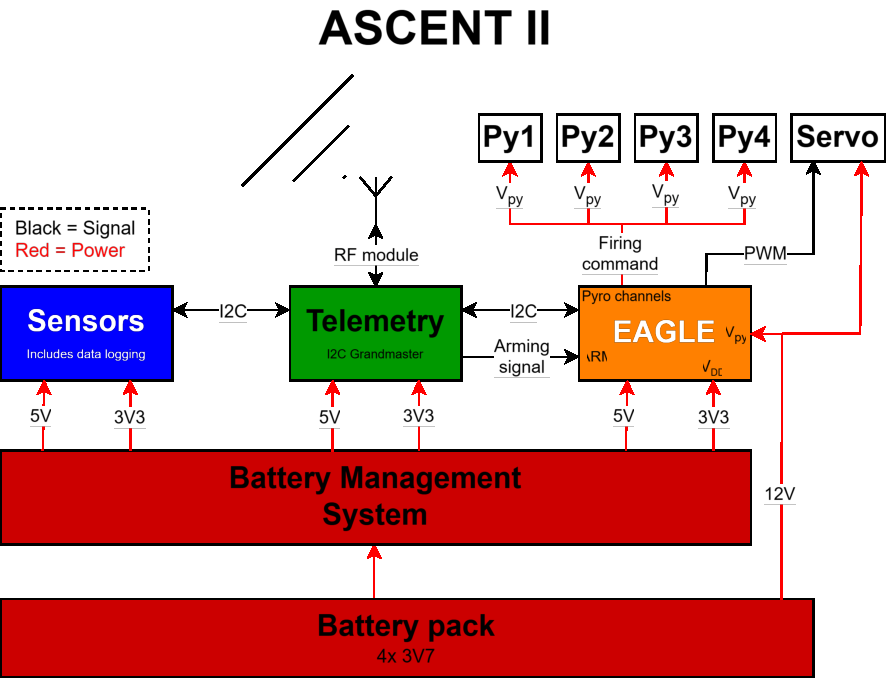
\includegraphics[width=.7\textwidth]{ASCENT II Architecture.pdf}
	\caption{ASCENT II architecture}
	\label{fig:ASCENT_architecture}
\end{figure}

At the core of the "active" modules sits the telemetry module which serves as the grandmaster\footnote{Each module has two I2C channels. "Grandmaster" refers to the master of the channel over which the modules communicate with each other, "master" refers to the channel which each module uses "locally" for communcation with e.g. sensors.} in the I2C communication interface. This was chosen since it will be receiving and transmitting all necessary flight data to the ground station as well receive and manage all incoming commands from the ground. It initiates communication with the other modules when it is ready to receive data to be transmitted using so called "interrupts" on the I2C channel. This causes the slave module to interrupt its current software for a very short amount of time to answer the call from the telemetry module. Since the modules run asynchronously\footnote{They run at different loop timings and are not synchronized}, there would otherwise be a chance of packet loss due to overbuffering. This could be caused by one module sending data quicker than the other communication partner can receive/read said data. Additionally, this also avoids the possibility of multiple modules trying to communicate over the same channel at once, which would result in the loss of all packets on the channel, due to the nature of I2C half-duplex architecture. One of the before mentioned commands is the arming signal and the deployment commands. As part of the requirements in chapter \ref{chap:Requirements}, it is necessary to provide more than one step in order to be able to deploy any kind of energetics on the launch pad. Without an active arming signal, which is given by a user-command\footnote{Has to be sent by a human-in-the-loop}, EAGLE is not able to fire any pyro-channel and therefore deploy any parachutes.\\
The sensor modules' primary objective is collecting and logging all the critical flight data that can be used for flight analysis after touchdown. It not only collects data about altitude and internal pressures, but also about the GNSS position and bending loads on the rocket using strain gauges. It also receives essential data about the state of flight from EAGLE using the UART communication protocol so that said data can also be logged. The logging happens on an SD-card as well as a flash chip. The latter being necessary for a hard touchdown as IC's are not prone to cracking under shock, whereas SD-cards can easily crack under shock loads.\\
The battery managements system is ASCENT II's only "passive" module, meaning that there is no software or microcontroller involved. It only utilizes passive elements such as DC-DC voltage converters, capacitors and resistors to execute its function. Its main objective is to down-regulate the incoming 14.8\,V from the battery pack to 3.3\,V and 5\,V, which are then used by the other modules to power things such as microcontrollers and sensors (3.3\,V) and such as the telemtry module (5\,V). On top of that, it smooths out voltage spikes by using a combination of resistors and capacitors.\\
The last of ASCENT II's modules is EAGLE, which controls parachute deployment and airbrake actuations. It also features its own set of sensors in order to make it independent of the sensor modules. This was done, because the only way left to communicate between the two modules was UART (due to lack of I2C channels) or SPI. The latter being considered to complex to be implemented at the time and the other being considered significantly slower than I2C in terms of communication speed, which is not reliable enough for real-time decision making.\\
In total, ASCENT II consists of five PCB's (2 Sensor modules), which are all individually designed along a certain design standard and PCB concept, which will be further discussed in subchapter \ref{sec:PCB_concept}.

\subsection{PCB concept} \label{sec:PCB_concept}
In order to ensure the modularized design and having a consistent designs across all modules, a PCB concept was implemented. The concept, as seen in figure \ref{fig:PCB_concept}, consists of some standard component that should included in every module. One of these components are the two pin connectors on the left and right of the PCB. These are the main connections between the modules and carry signals and voltage supply over common pins. Additionally, there is a programming interface on the bottom left of the top view, which can I either be connected to a commonly used USB to UART converter or a UPDI converter, which can both be used for programming the microcontroller, depending on which protocol it supports. To the right of said interface, there is two status LED's. One of them, is single color LED, whilst the other is a RGB LED. The single color LED can be used to show simple debugging steps, like that the microcontroller is running and executing its software. The RBG LED is supposed to display the status of the module. This could be something like green = running, red = error and other colors indicating what part of the software is being executed. These LED's main purpose is debugging and troubleshooting with visual feedback, which would be crucial during a launch campaign, where any kind of mistake should ideally be caught before final integration.\\
For integration purposes, the PCB also has standardized mounting holes, which can only be mounted in one specific way. That way, no PCB can be mounted incorrectly leading to the pins on the connector to be swapped around. When stacked, the PCB's are connected by the pin connectors and by threaded spacers which screw together through the mounting holes.\\
All of these standard features were either proven during or a learning of SPROG's inaugural launch.

\begin{figure}[H]
	\centering
	\captionsetup{font=footnotesize}
	\subfigure[Top view]{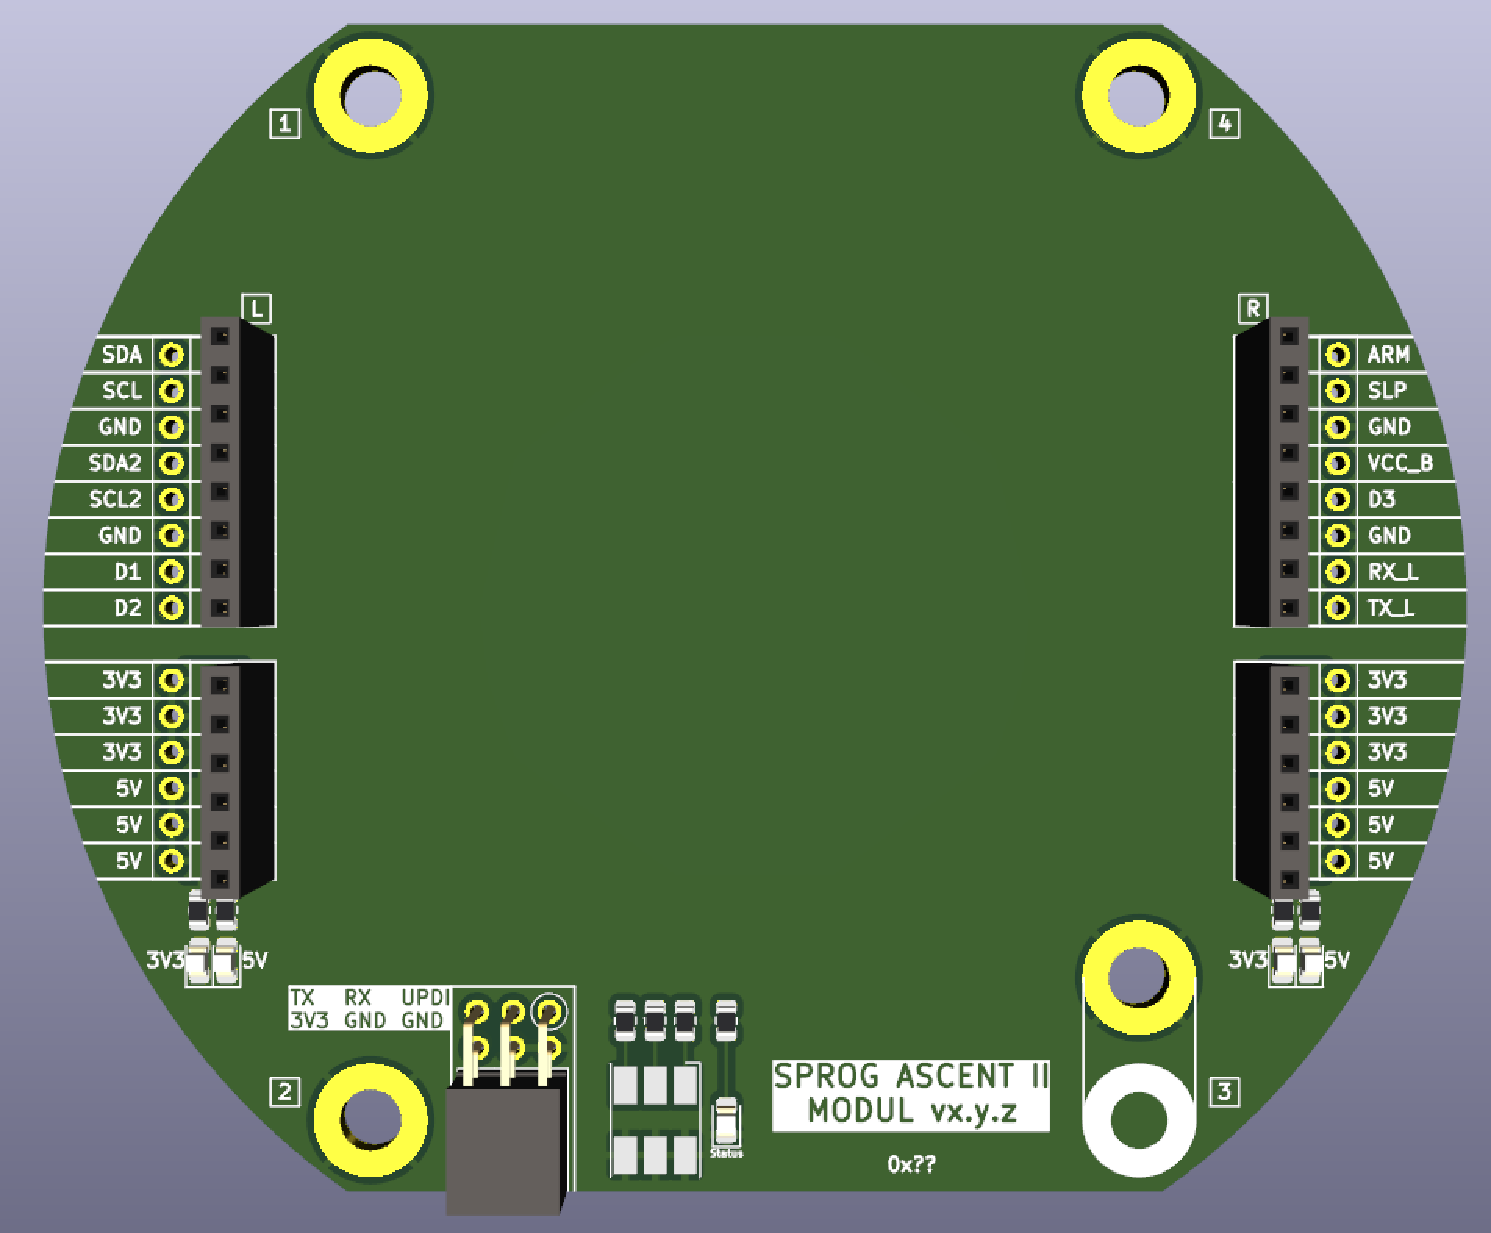
\includegraphics[width=0.48\textwidth]{PCB-conccept-top.pdf}}
	\hfill
	\subfigure[Bottom view]{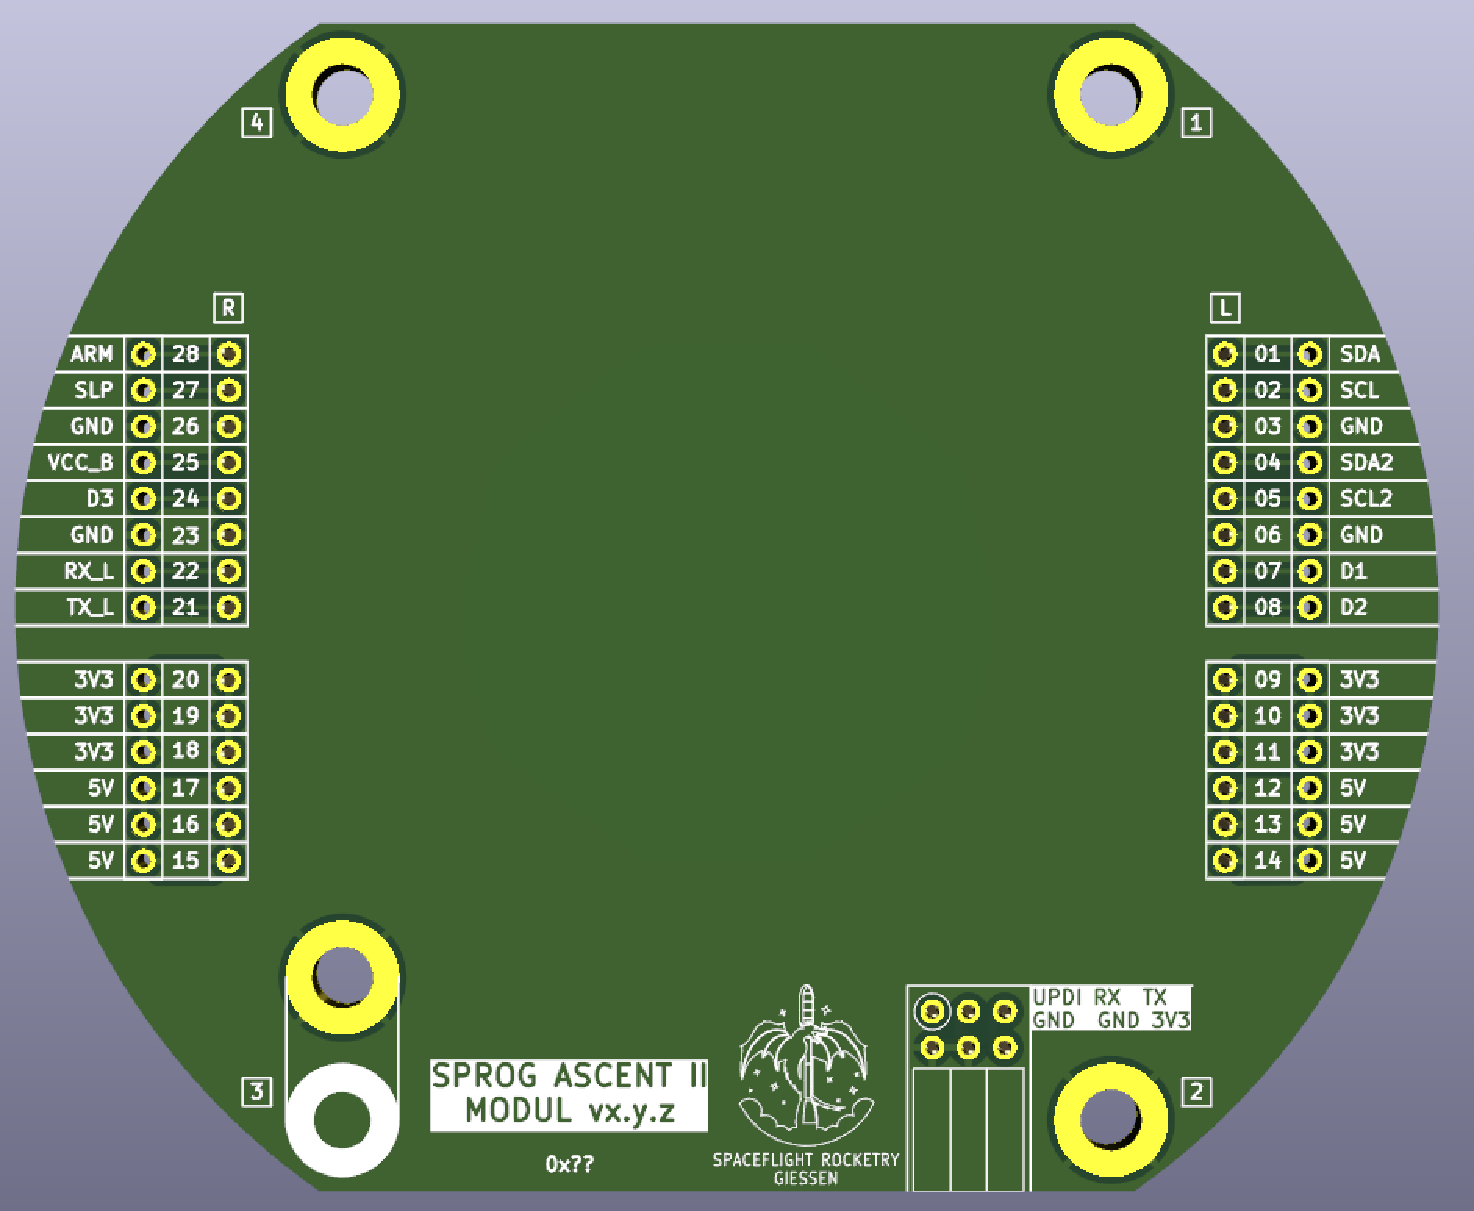
\includegraphics[width=0.48\textwidth]{PCB-conccept-bottom.pdf}}
	\caption{PCB concept}
	\label{fig:PCB_concept}
\end{figure}

\subsection{EAGLE Architecture}
EAGLE's architecture, which is shown in figure \ref{fig:EAGLE_architecture} slightly varies from that of the other modules. This comes down to the fact that EAGLE is designed to handle a broader variation of system i.e. airbrakes, parachute deployment and staging. To keep up reliability and minimize the effect of external influences, EAGLE does most of the flight computers tasks independently. This also includes its own set of sensors. The amount of sensors is based on the redundancy requirement in EuRoC's. For this reason, every type of sensor, except for the inertial measurement unit (IMU), has a redundant partner from an entirely different manufacturer. This is done so that no systematic issues of the sensor influence both readings, creating a more robust infrastructure. An IMU collects acceleration data (similar to the accelerometers) but also collects rotation speed. Since there are already two accelerometers, adding another acceleration reading will improve accuracy of the processed signal, but will not have a big impact of overall system reliability. The reason it was still added is purely for its capability to retrieve the rotation speed, which was added in case such a measurement might be needed in the future. In addition to sensors, it became apparent that additional input and output (IO) ports were needed. For this reason a (GP-)IO multiplexer was added, which added another 16 IO's to the already existing IO's of the microcontroller.\\ 
To communicate and process the data from the sensors and multiplexer, EAGLE features its own microcontroller, which uses its secondary I2C port to communicate with the sensors with itself as the master and each sensor as its slave. Furthermore, it communicates with the telemetry module using I2C where it acts as the slave of the grandmaster. If the arming signal was given by the telemetry module, it was possible for the main control unit (MCU) to send a voltage signal to the pyro-channels, which would lead to the firing current to be released. On top of that, the MCU can also send sensing voltages, which would not be high enough to ignite the pyrotechnics, to detect the current running through the system. If it was then able to detect any form of current, it was clear that a pyrotechnic igniter was installed and continuity on the channel was present. The MCU is also capable of sending PWM signals to a servo that would actuate the airbrakes.\\
During the development of ASCENT I, it was discovered that requiring a middle man to decode USB to UART signals in order to program the MCU, was time consuming and complex, because it required you to put both systems on the same power and ground reference, which made programming labour intense. To avoid this, with this iteration, EAGLE features a USB-C interface that includes all features of the USB to UART converter, which would let you read data from the MCU and program it with one interface, without connecting any additional wires.\\
There are also some external connections. These include the before mentioned I2C connection to the grandmaster, with EAGLE acting as its slave. It also includes the arming signal, without EAGLE is physically incapable of firing the pyro-channels. EAGLE also gets its main voltage supply $V_\text{dd}$, a 3.3\,V connection and the supply voltage for the pyrotechnics $V_\text{py}$ from external connections\footnote{Any external connection mentioned in this subchapter refers to connections coming from the pin connectors}. $V_\text{dd}$ and $V_\text{py}$ are then internally routed to the pyro-channels where they are used.

\begin{figure}[H]
	\centering
	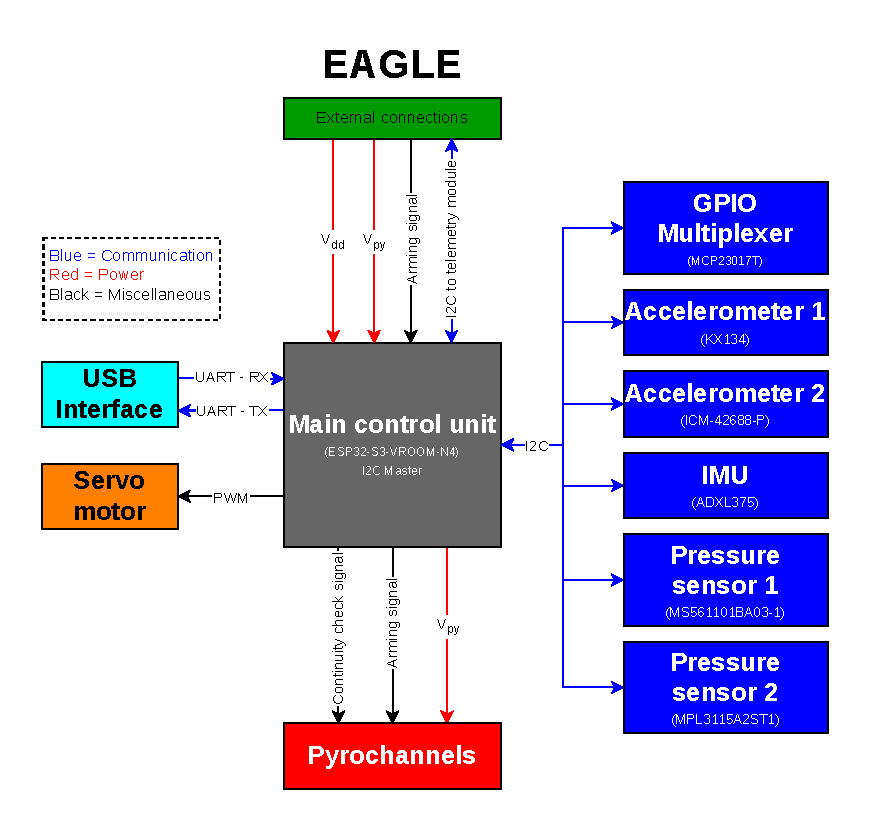
\includegraphics[width=.7\textwidth]{EAGLE Architecture.pdf}
	\caption{EAGLE architecture}
	\label{fig:EAGLE_architecture}
\end{figure}




\section{Software Architecture}
With EAGLE being in charge for many systems that would be considered saftey-critical, it is imperitive that the software is just as reliable as the hardware. Any unexpected behaviour can - in the worst-case scenario - cause a catastrophic failure, which could result in the loss of the rocket or damage to person and property. The overall architecture and decisions that led to this architecture will be highlighted in this subchapter.

\subsection{State machine}
EAGLE's software is based on the concept of a state machine which was introduced in subchapter \ref{sec:state_machine}. The reason it was chosen as the architecture is due to the predictability and simplicity. On top of that, a rockets trajectory can be split into certain milestones or states (as discussed in subchapter \ref{sec:trajectory}). EAGLE's state machine consists of eight states, which are shown in figure \ref{fig:Software_architecture}. The states consist of "Pad idle" (0), "Initialized" (1), "Armed" (2), "Boost phase" (3), "Coasting" (4), "Apogee" (5), "Main deployment" (6), "Landed" (7) and "Abort" (8). Each state is assigned a number as part of an enumeration, which maps number values to strings for easier use in the software. The numbers of each state are represented in parentheses.

\begin{figure}[H]
	\centering
	\includegraphics[width=\textwidth]{software architecture.pdf}
	\caption{Software architecture}
	\label{fig:Software_architecture}
\end{figure}

"Pad idle" is the starting state of the state machine. It is the default state that is assumed when EAGLE is powered on. At this stage, communication to the sensors is established by running an "I2C scanner", which sends a handshake (signal) to all 255 possible I2C addresses and waits for a response. If a response is received, communication to the sensor is considered established. Additionally, continuity of the pyro channels is checked. It detects a sensing current going through the pyrotechnic igniters. Detecting the sensing current on the minus port of the pyro channel implicates that the electrical circuit is closed, indicating a connected igniter. Each igniter can be tested individually by cycling through the individual pyro channels. At this point, anything that is off nominal would lead to an abort or recycle. Whilst EAGLE is made of many redundancies, it is unwise to launch with the knowledge that these redundancies have already been used. During this phase the vehicle is still unarmed and can quickly be taken down for inspection, which is why it makes sense to abort the launch should any abnormalities be found.\\
"Initialized" indicates that the microcontroller has successfully established communication with all sensors and peripherals, whilst also confirming that igniters are connected. In this state, the continuity to the igniters is still continuously checked, while waiting for the armed command from the telemetry via I2C.\\
Once the arming has been confirmed EAGLE enters the "Armed" state. In this state only continuity and liftoff detection are being checked for. Similarly to the prior states, any abnormalities on the continuity would result in an abort. Liftoff is detected by using the accelerometer data to detect a spike in acceleration, which would only happen when the booster is producing its main thrust. After liftoff, continuity will no longer be checked as the main objective is no longer to catch abnormalities, but to perform the main flight logic.\\
As already discussed in subchapter \ref{sec:trajectory}, a key characteristic of booster burnout is an acceleration of $\approx9.81\,\frac{\text{m}}{\text{s}^2}$ on the axis perpendicular to the ground. When this is detected, the software enters the coasting phase. During this phase, staging will be initiated (if the rocket is two staged) and the airbrake logic will be executed, because it is the only phase in the ascent, where only gravitation and aerodynamics dictate the flight.\\
The "Apogee" state runs the logic required to deploy the drogue parachute. This is dictated by the EuRoC rules as shown in subchapter \ref{sec:euroc}. At apogee, pyro channel 1 would be set to high igniting the first set of pyro charges. Additionally, there is logic which detects drogue deployment. If drogue deployment is not detected after a certain time, pyro channel 2 will be set to high, to ignite the secondary, redundant pyro charge for the drogue. Even without confirmed deployment, it constantly checks the current altitude versus the setpoint set for main parachute deployment.\\
"Main deployment" is essentially the same as apogee, but it used pyro channel 3 as primary and channel 4 as redundant igniter. Whilst this state follows the pyro state, it is not necessary to have a confirmed drogue deployment in order to try to deploy the main parachute. This is due to the fact, that a false negative on the confirmation is possible and it should not prevent the main parachute from deploying. On top of that, there is no downside to trying to deploy main parachute. Although there are low chances that the main would deploy without the drogue, it is not impossible, so it is reasonable to attempt the deployment.\\
As a last step, the vehicle enters the "Landed" state, which tells the telemetry to un-arm the pyro channels, so the rocket can safely be approached. It also tells the telemetry to initiate recovery procedures such as activating a beeper and power down systems to allow for maximum sending time of the touchdown location.\\
If there are any off nominal reports during the setup process, the "Abort" state may be entered, which tells the operator on the ground to hold the launch. However, this state does not have the capabilities to prevent the launch other than advice the operator to stand down. From an abort state, the telemetry can be used to make a decision whether to recycle the attempt, which means that the state machine would remotely be set back into the "Pad Idle" state by an operator or whether to abort the launch attempt and take the rocket off of the launch rail.

\subsection{State transitions}
Each transition between states is governed by one or more boolean trigger conditions derived from sensor readings and system checks. Table \ref{tab:setup_state_transitions} and table \ref{tab:flight_state_transitions} specify these conditions for the setup phase and flight phase, respectively. Within these tables, a dash ("–") denotes a don't-care condition: the corresponding flag has no influence on whether the transition occurs, and may hold either value.\\
Following power-up, the system resides in the initial setup/pad idle state (0). If both the sensors established and continuity flags evaluate to TRUE, initialization is considered complete and the system transitions to the initialized state (1), independent of the armed flag's state at that point. Conversely, if both flags are FALSE, setup is deemed to have failed and the system transitions directly to the abort state (8).\\
From state 1, the system remains unarmed as long as continuity is maintained and the armed flag is FALSE (transition $1\rightarrow1$). If the armed flag becomes TRUE while continuity is still present, the system transitions to the armed state (2). Should continuity be lost at any point while in state 1, the system transitions to the abort state (8), regardless of the other flags.\\
State 2 behaves analogously with respect to continuity: the system remains in state 2 as long as continuity is present ($2\rightarrow2$), and transitions to the abort state (8) if continuity is lost.\\
Once setup completes successfully, the system enters the armed state (2), from which it transitions to the boost state (3) upon detection of liftoff. (As shown in table \ref{tab:flight_state_transitions}, state 2 additionally reverts to the abort state (8) if continuity is lost prior to liftoff).
If the system enters an abort state, an operator on the ground may decide to abort the launch attempt or to recycle the state machine, forcing it back into the pad idle state, from where operations would start over again.\\
After detecting liftoff, the system monitors for booster burnout, apogee and main deployment. Each variable can lead to a different transition, as it is possible that either one of these steps is missed. However, it is important that EAGLE remains capable of deploying parachutes even if one or more events have been missed. For that reason, detecting apogee or main deployment altitude, would result in the state transition into the apogee ($3\rightarrow5$) or main deployment ($3\rightarrow6$) state. If the event monitoring is nominal, the coasting phase ($3\rightarrow4$) would be entered. Im the off-nominal case, the coasting phase would be skipped and all airbrake actuation would not be executed. This is done to ensure EAGLE's main objective, which is the successful and safe recovery of the rocket.\\
Analogous to the boost state, the system can jump into multiple outcomes, in this case into apogee ($4\rightarrow5$) and into main deployment ($4\rightarrow6$). This is done for the same reason of being able to control the parachutes even if an event has failed to get noticed.\\
When in the apogee state, the state machine has the nominal case of detecting main deployment ($5\rightarrow6$). However, there is still a chance that such an event would be missed, in which case the rocket would fall to the ground under drogue parachute, which would cause a relatively high impact speed. In this case, the rocket still needs to be able to inert (unarm) itself, if it survived the impact and therefore needs to be able to detect the landing, which would cause a transition into the landed state ($5\rightarrow7$).\\
If the vehicle does deploy the main parachute or at least enters state 6, it can only transition into landed as it is the last step in the flight sequence of events.\\
The events "apogee detected", "main parachute altitude detected" and "landing detected" can each be redundantly triggered by a ground operator command or by timeout. When EAGLE detects liftoff it starts timers which evaluate if an event could have been reached based on timings from simulations. So even if EAGLE was to not detect apogee or main deployment and still managed to survive the impact, a timer would cause the rocket to inert itself. Similarly, this serves as backup for missed apogee detecting by the sensor values.\\

\subsection{PID Controllers}

\subsection{Internal data processing}

\subsection{Implementation}
Similarly to the state machine, the software is split into a main function and a setup code. The key difference is that the setup code is only called once, whereas the main function is a loop as seen in the code example \ref{code:top_level} . This is part of the arduino framework which was chosen for this project because of its wide range of open-source libraries, which could be used for reading sensors or communicating via UART or I2C.\\

\begin{lstlisting}[caption={Top level code design}, label={code:top_level}]
void setup{
	//runs setup state machine	
	if(liftoff detected && continuity detected)
		state = boost; //start main loop
}
int main {
	while(state != landed){
		//runs flight state machine
		if(execution time > set execution time)
			skip.to.next.iteration;
	}
}
\end{lstlisting}

Because of the time critical nature of the system, it is important that the software runs deterministic i.e. that it runs its main loop in a pre-defined amount of time. This is important, to avoid unexpected behavior. This can be enforced by e.g. using interrupts, which completely stops the loop iteration if this set amount of time has been exceeded. The time for the loop to finish is set by creating a statistic about how long the loop takes to run once over multiple iterations, but can also be pre-defined as a requirement. In this case, it was decided to base it on the average execution time, because whilst it is important to have a deterministic code, parachute deployment may happen within the vicinity of apogee and the main deployment altitude as discussed in subchapter \ref{sec:euroc_rules}.\\

The implementation of the state machine is done by using an enumeration, a list of string values that are assigned to numbers, for abstracting the states, which in turn makes the code more readable. In the main loop, a switch-case statement, essentially a large number of if-else-statements, is executed in every iteration (as shown in code example \ref{code:state_machine}). The main loop only starts executing logic, once the setup process is complete, liftoff was detected and the state has been changed to "boost". The switch-case statement checks which state is currently active and only executes that specific state's logic.

\begin{lstlisting}[caption={States enumeration}, label={code:enum}]
enum States {
	pad_idle = 0,
	initialized = 1,
	armed = 2,
	boost = 3,
	coast = 4,
	apogee = 5,
	main_deploy = 6,
	landed = 8
};
\end{lstlisting}

\begin{lstlisting}[caption={Flight state machine}, label={code:state_machine}]
while(state != landed){
	getSensorData(); //retrievs sensor data
	switch(state) {
		case boost:
			//execute burnout monitoring
			break;
		case coast:
			//execute airbrake and staging logic
			break;
		case apogee:
			//execute drogue deployment logic
			break;
		case main_deploy:
			//execute main deployment logic
			break;
		case landed:
			//execute post-touchdown/inerting logic
			break;
		default:
			//do nothing until a known state is set by the setup state 
			//machine
	}
}
\end{lstlisting}

In each state, outputs are set and the state transition triggers are evaluated. If a transition trigger is detected, the global state variable "state" (can be changed and accessed by all functions) is changed and the respective case is executed. A check for a state transition trigger can look like the following:

\begin{lstlisting}[caption={State transition logic}, label={code:state_transition}]
switch(state) {
	case boost:
	//boost state logic
	if(burnout detected)
		state = burnout;
	break;
\end{lstlisting}

Because of the break statement, the switch-case statement finishes for this iteration and will assume the burnout state in the next iteration.\\
In order to be able to process data within each case, sensor data has to be retrieved. This is done, before calling the switch-case statement, because every state needs the sensor data and it therefore makes the code more readable. In this sensor reading function, all 5 sensors are called and read. Afterwards, the data gotten from these sensors is processed using common data filters to narrow down the error in data calculations. On top of that, multiple sources of the same data will be calculated into one single data point, so that the case only has to call the processed data and does not have to do any advanced arithmetics.

\newpage

\chapter{Preliminary design phase}
Based on prior experience at SPROG, it was decided that each system would need to go through a preliminary design phase during which the requirement and architecture that were defined were to be tested for feasibility. This is done, to ensure that no resources are lost to small mistakes, which were not detected, because of a lack of knowledge or experience. This was an issue that poised SPROG's early stage developments. During the development of ASCENT I, PCB's were designed and ordered early on with minor to major design flaws costing the association time and resources, which were limited during that time due to the young age of the group. This phase was mostly about understanding and selecting the correct sensors and confirm the design on basic open questions. For example, the sensor module phased the question whether to use a built in antenna for the GNSS module or an external antenna. The only relevant open question during this phase was the selection of sensors. The process that were taken to limit the amount of unknowns in the PCB design phase, will be illuminated in this chapter.

\section{Process}
The first step in the preliminary design phase is the selection of components. The requirements dictate the amount of sensors and overall architecture but not which components to use exactly. Therefore, the first major step is to decide on the sensors that were to be used. However, there is no final decisions at this point. This is because each selected sensor had to go through initial testing on breakout boards and had to match certain expectations, which were evaluated during this process.

\section{Component selection}
The requirements and the consequent architecture required five sensors in total: Two accelerometers, two pressure sensor and one inertial measurement unit (IMU) to detect all data necessary for EAGLE's operation. To decide 

\section{Component evaluation}


\chapter{PCB Design - CanSat version}





\section{Design Evaluation and Revision}

\newpage


\chapter{PCB Design - ASCENT II}


\newpage

\chapter{Verification and Testing}

\newpage


\chapter{Discussion}

\iffalse
\chapter{Selection of components}
The components of the PCB make up the most integral part of this system as all decisions and signals are relying on high quality data with low noise. Therefore, a significant amount time was spent researching a multitude of sensors and other components. As mentioned in, the board will feature five sensors and a microcontroller powerful enough to handle all the data. The most important requirements for these is an operating voltage of either 3.3V or 5V as that is the voltage that is being supplied by the PSU.

\section{Microcontroller}
The microcontroller is the heart of all operations and needs to be the most reliable component on the PCB. It collects all the data from the sensors and distributes it to the telemetry system and data storage as well as fire pyro-channels and actuate the servos and be able to read analogue signals. Therefore, the selected microcontroller needs a wide range of pin-types.

\subsection{AVR128DB64}
The AVR128DB64 was the first choice solely based on past experience and ease of programming. It has an easy to understand pinout and 64 pins and runs on the arduino framework. The AVR128DB28 (same family of controllers) has been used in a previous telemetry system meaning there was a lot of experience using this type of microcontroller. Additionally, it allows communication via SPI, UART and I2C (commonly used communication protocols). The latter being used for communication with all sensors and between the communication with the telemetry subsystem. It also featured a relatively new programming protocol called "UPDI", which only requires one pin for programming instead of two dedicated UART ports like other microcontrollers, making programming substantially easier.\\
In hindsight, there should have been less emphasize on past experiences as they allowed for an oversight on the computing power of the chip, which is arguable the most important characteristic. After connecting and testing multiple sensors to the microcontroller, it was discovered the RAM overflowed with data during the first loop, rendering the microcontroller useless for usage in EAGLE.

\subsection{ESP32-S3-Vroom-N4-1u}
After running into issues with the AVR128DB64 a team member of the electronics working group within the association suggested to test the ESP32 as it is a dual-core microcontroller and has more RAM available. It also features all common communication protocols, but needs to be programmed using UART, rendering two pins unusable for any other purposes. The programming also needs to additional pins called "EN" and "IO0" which need to be pulled to GND in a specific sequence to put the microcontroller into the so called "programming mode". However, it did feature a D+ and D- pin meaning a USB interface can easily be connected for programming and data-reading. In addition to that, it is an IC meaning that it has additional features such as an built-in WiFi module and antenna. To save space it was decided to use the "-1u" version, because that means that the ESP32 would come without an antenna but with a coax-connector. However, all of this came at the cost of the arduino framework as ESP32s run on their own firmware and framework. In some cases however, the ESP32 is capable of running arduino code, meaning that the code only needs to be adapted slightly.\\
For those reasons, the ESP32-S3-Vroom-N4-1u was chosen as the microcontroller for EAGLE.
\fi

\newpage
\printbibliography %Prints bibliography

\setcounter{page}{1}
\pagenumbering{Roman}
\chapter{Appendix}

\section{Tables}

\subsection{State transition truth tables} \label{adx:State_transitions}

\begin{table}[H]
	\captionof{table}{EAGLE setup state transitions}	
	\label{tab:setup_state_transitions}
	\centering
	\begin{tabular}{|c|l||c|c|c|c|} \hline		
		\multicolumn{2}{|c||}{\textbf{Transition description}} & \multicolumn{4}{c|}{\textbf{Transition trigger}}\\ \hline
		\textbf{Transition} & \textbf{Cause} & \textbf{Sensors established} & \textbf{Continuity} & \textbf{Armed} & \textbf{Recycle} \\ \hline \hline
		$0\rightarrow1$ & Initialization complete & TRUE & TRUE & -\tablefootnote{"-" means that the state of this flag is unimportant for the transition trigger} & FALSE\\ \hline
		$0\rightarrow8$ & Setup failed & FALSE & FALSE & - & FALSE \\ \hline
		$1\rightarrow1$ & No change & - & TRUE & FALSE & FALSE \\ \hline
		$1\rightarrow2$ & Armed signal & - & TRUE & TRUE & FALSE \\ \hline
		$1\rightarrow8$ & No continuity & - & FALSE & - & FALSE \\ \hline
		$2\rightarrow2$ & No change & - & TRUE & FALSE & FALSE \\ \hline
		$2\rightarrow8$ & No continuity & FALSE & - & - & FALSE \\ \hline
		$8\rightarrow0$ & Recycle command & - & - & - & TRUE \\ \hline
	\end{tabular}
\end{table}
	
\begin{sidewaystable}
	\captionof{table}{EAGLE flight state transitions}	
	\label{tab:flight_state_transitions}
	\centering
		\begin{tabular}{|c|l||c|c|c|c|c|} \hline
			\multicolumn{2}{|c||}{\textbf{Transition description}} & \multicolumn{5}{c|}{\textbf{Transition trigger}}\\ \hline
			\textbf{Transition} & \textbf{Cause} & \textbf{Liftoff detected} & \textbf{Burnout detected} & \textbf{Apogee detected} & \makecell{\textbf{Main deploy}\\ \textbf{setpoint detected}} & \textbf{Landing detected} \\ \hline \hline
			$2\rightarrow3$ & Liftoff detected & TRUE & - & - & - & - \\ \hline
			$3\rightarrow3$ & No change & - & FALSE & - & - & - \\ \hline
			$3\rightarrow4$ & Burnout detected & - & TRUE & - & - & - \\ \hline
			$3\rightarrow5$ & Apogee detected & - & - & TRUE & FALSE & - \\ \hline
			$3\rightarrow6$ & Main deploy setpoint detected & - & - & FALSE & TRUE & - \\ \hline
			$4\rightarrow4$ & No change & - & - & FALSE & FALSE & -\\ \hline
			$4\rightarrow5$ & Apogee detected & - & - & TRUE & - & -\\ \hline
			$4\rightarrow6$ & Main deploy setpoint detected & - & - & FALSE & TRUE & -\\ \hline
			$5\rightarrow5$ & No change & - & - & - & FALSE & -\\ \hline
			$5\rightarrow6$ & Main deploy setpoint detected & - & - & - & TRUE & - \\ \hline
			$6\rightarrow6$ & No change & - & - & - & - & FALSE\\ \hline
			$6\rightarrow7$ & Landing detected & - & - & - & - & TRUE\\ \hline
		\end{tabular}
\end{sidewaystable}

\newpage

\subsection{Sensor characteristics}

\begin{center}
	\captionof{table}{Inertial Measurement Unit(IMU) characteristics Nr.1}	
	\label{tab:sensor_imu1}
	\begin{adjustbox}{width=1.15\textwidth}		 
		\begin{tabular}{|r||c|c|c|c|c||c|c|c|c|} \hline		
			& \multicolumn{5}{c||}{\textbf{BMI160}} & \multicolumn{4}{c|}{\textbf{MPU6500}}\\ \hline
			
			\rowcolor{light grey} $Accelerometer Specs$ & \multicolumn{5}{c}{} & \multicolumn{4}{c}{} \\ \hline \hline
			
			\textbf{Measurement Range} & 2\,g & 4\,g & 8\,g & \multicolumn{2}{c||}{16\,g}& 2\,g & 4\,g & 8\,g & 16\,g\\ \hline
			
			\textbf{Output Resolution} & \multicolumn{5}{c||}{16\,bits} & \multicolumn{4}{c|}{16\,bits}\\ \hline
			
			\textbf{Sensitivity} (Typical) & 16384\,$\frac{\text{LSB}}{\text{g}}$ & 8912\,$\frac{\text{LSB}}{\text{g}}$ & 4096\,$\frac{\text{LSB}}{\text{g}}$ & \multicolumn{2}{c||}{2048\,$\frac{\text{LSB}}{\text{g}}$} & 16384\,$\frac{\text{LSB}}{\text{g}}$ & 8192\,$\frac{\text{LSB}}{\text{g}}$ & 4096\,$\frac{\text{LSB}}{\text{g}}$ & 2048\,$\frac{\text{LSB}}{\text{g}}$\\ \hline
			
			\multirowcell{2}{\shortstack[r]{\textbf{Sensitivity change}\\ \textbf{due to temperature}}} & \textbf{x} & \multicolumn{2}{c|}{\textbf{y}} & \multicolumn{2}{c||}{\textbf{z}} & \textbf{x} & \multicolumn{2}{c|}{\textbf{y}} & \textbf{z}\\ \cline{2-10}
			
			& \multicolumn{5}{c||}{$\pm0.03\,\frac{\%}{\text{°\text{C}}}$} & \multicolumn{4}{c|}{$\pm0.026\,\frac{\%}{\text{°\text{C}}}$}\\ \hline
			
			\textbf{0g Offset} & \multicolumn{5}{c||}{$\pm0.04\,\text{g}$} & \multicolumn{4}{c|}{$\pm0.06\,\text{g}$}\\ \hline
			
			\textbf{Noise} & \multicolumn{5}{c||}{$\pm1.8\,\text{mg-rms}$} & \multicolumn{4}{c|}{Low Noise Mode: $\pm300\,\frac{\text{\textmu g}}{\sqrt{\textbf{Hz}}}$}\\ \hline
			
			\multirowcell{2}{\textbf{Operating Voltage} $V_\text{s}$/$V_\text{DD}$} & \textbf{Min} & \multicolumn{3}{c|}{\textbf{Typical}} & \textbf{Max} & \textbf{Min} & \multicolumn{2}{c|}{\textbf{Typical}} & \textbf{Max}\\ \cline{2-10}
			
			& 1.71\,V & \multicolumn{3}{c|}{3.0\,V} & 3.6\,V & 1.71\,V & \multicolumn{2}{c|}{1.8\,V} & 3.45\,V\\ \hline
			
			\textbf{Interface Voltage} $V_\textbf{DDIO}$ & 1.2\,V & \multicolumn{3}{c|}{2.4\,V} & 3.6\,V & 1.71\,V & \multicolumn{2}{c|}{1.8\,V} & 3.45\,V\\ \hline
			
			\multirowcell{2}{\textbf{Output Data Rate} (ODR)} & \multicolumn{2}{c|}{\textbf{Min}}& \multicolumn{3}{c||}{\textbf{Max}} & \multicolumn{2}{c|}{\textbf{Min}}& \multicolumn{2}{c|}{\textbf{Max}}\\ \cline{2-10}
			
			& \multicolumn{2}{c|}{12.5\,Hz} & \multicolumn{3}{c||}{1600\,Hz} & \multicolumn{2}{c|}{4\,Hz} & \multicolumn{2}{c|}{4000\,Hz}\\ \hline
			
			\multirowcell{2}{\textbf{Current Consumption}} & \multicolumn{2}{c|}{\textbf{Accelerometer}} & \textbf{Gyroscope} & \textbf{Both}(On) & \textbf{None}(Stby) & \textbf{Accelerometer} & \textbf{Gyroscope} & \textbf{Both}(On) & \textbf{None}(Stby)\\ \cline{2-10}
			
			& \multicolumn{2}{c|}{300\,\textmu A} & 900\,\textmu A & 990,\textmu & 10\,\textmu A & 0.45\,mA & 3.2\,mA & 3.4\,mA & 1.6\,mA\\ \hline
			
			\multirowcell{2}{\textbf{Power Consumption}} & \multicolumn{5}{c||}{\textbf{For Typical $V_\text{DD}=3.0\,$V}} & \multicolumn{4}{c|}{\textbf{For Typical $V_\text{DD}=1.88\,$V}}\\ \cline{2-10}
			
			& \multicolumn{2}{c|}{0.90\,mW} & 2.70\,mW & 2.97\,mW & 0.03\,mW & 0.81\,mW & 5.76\,mW & 6.12\,mW & 2.88\,mW\\ \hline
			
			\textbf{Temperature Range} & \multicolumn{5}{c||}{-40\,...\,+85\,°C} & \multicolumn{4}{c||}{-40\,...\,+85\,°C}\\ \hline\hline 
			
			\rowcolor{light grey} $Gyro Specs$ & \multicolumn{9}{c||}{}\\ \hline\hline
			
			\textbf{Measurement Range} & 125\,$\frac{\text{deg}}{\text{s}}$ & 250\,$\frac{\text{deg}}{\text{s}}$ & 500\,$\frac{\text{deg}}{\text{s}}$ & 1000\,$\frac{\text{deg}}{\text{s}}$ & 2000\,$\frac{\text{deg}}{\text{s}}$ & 250\,$\frac{\text{deg}}{\text{s}}$ & 500\,$\frac{\text{deg}}{\text{s}}$ & 1000\,$\frac{\text{deg}}{\text{s}}$ & 2000\,$\frac{\text{deg}}{\text{s}}$\\ \hline
			
			\textbf{Sensitivity} & 262.4\,$\frac{\text{LSB}}{\frac{\text{deg}}{\text{s}}}$ & 131.2\,$\frac{\text{LSB}}{\frac{\text{deg}}{\text{s}}}$ & 65.6\,$\frac{\text{LSB}}{\frac{\text{deg}}{\text{s}}}$ & 32.8\,$\frac{\text{LSB}}{\frac{\text{deg}}{\text{s}}}$ & 16.4\,$\frac{\text{LSB}}{\frac{\text{deg}}{\text{s}}}$ & 131\,$\frac{\text{LSB}}{\frac{\text{deg}}{\text{s}}}$ & 65.5\,$\frac{\text{LSB}}{\frac{\text{deg}}{\text{s}}}$ & 32.4\,$\frac{\text{LSB}}{\frac{\text{deg}}{\text{s}}}$ & 16.4\,$\frac{\text{LSB}}{\frac{\text{deg}}{\text{s}}}$\\ \hline
			
			\makecell{\textbf{Sensitivity Change}\\\textbf{Due to temperature}} & \multicolumn{5}{c||}{$\pm0.02\,\frac{\%}{°\text{C}}$} & \multicolumn{4}{c|}{$\pm3\,\%$\tablefootnote[1]{maximum absolute offset}} \\ \hline
			
			\textbf{Zero-rate Offset} & \multicolumn{5}{c||}{$\pm3\frac{\text{deg}}{\text{s}}$} & \multicolumn{4}{c|}{$\pm5\frac{\text{deg}}{\text{s}}$} \\ \hline
			
			\textbf{Noise} & \multicolumn{5}{c||}{$0.07\frac{\text{deg}}{\text{s}}$-rms} & \multicolumn{4}{c|}{$\pm0.01\frac{\text{deg}}{\text{s}}$-rms} \\ \hline
		\end{tabular}
	\end{adjustbox}
\end{center}


\begin{sidewaystable}
	\captionof{table}{Inertial Measurement Unit(IMU) characteristics Nr.2}	
	\label{tab:sensor_imu2}
	\begin{adjustbox}{width=1.05\textwidth}		 
		\begin{tabular}{|r||c|c|c|c|c|c|c|c||c|c|c|c|c|c|c|c|c|} \hline		
			& \multicolumn{8}{c||}{\textbf{BMI160}} & \multicolumn{9}{c|}{\textbf{MPU6500}}\\ \hline
			
			\rowcolor{light grey} $Accelerometer Specs$ & \multicolumn{17}{c|}{}\\ \hline \hline
			
			\textbf{Measurement Range} & \multicolumn{2}{c|}{2\,g} & \multicolumn{2}{c|}{4\,g} & \multicolumn{2}{c|}{8\,g} & \multicolumn{2}{c||}{16\,g} & \multicolumn{2}{c|}{2\,g} & \multicolumn{2}{c|}{4\,g} & \multicolumn{2}{c|}{8\,g} & \multicolumn{2}{c|}{16\,g} & 32\,g\\ \hline
			
			\textbf{Output Resolution} & \multicolumn{8}{c||}{16\,bits} & \multicolumn{9}{c|}{16\,bits}\\ \hline
			
			\textbf{Sensitivity} (Typical) & \multicolumn{2}{c|}{16384\,$\frac{\text{LSB}}{\text{g}}$} & \multicolumn{2}{c|}{8912\,$\frac{\text{LSB}}{\text{g}}$} & \multicolumn{2}{c|}{4096\,$\frac{\text{LSB}}{\text{g}}$} & \multicolumn{2}{c||}{2048\,$\frac{\text{LSB}}{\text{g}}$} & \multicolumn{2}{c|}{16384\,$\frac{\text{LSB}}{\text{g}}$} & \multicolumn{2}{c|}{8192\,$\frac{\text{LSB}}{\text{g}}$} & \multicolumn{2}{c|}{4096\,$\frac{\text{LSB}}{\text{g}}$} & \multicolumn{2}{c|}{2048\,$\frac{\text{LSB}}{\text{g}}$} & 1024\,g\\ \hline
			
			\shortstack[r]{\textbf{Sensitivity change} \\ \textbf{due to temperature}} & \multicolumn{8}{c||}{$\pm0.005\,\frac{\%}{\text{°C}}$} & \multicolumn{9}{c|}{$\pm0.01\,\frac{\%}{\text{°C}}$} \\ \hline
			
			\textbf{0g Offset} & \multicolumn{8}{c||}{$\pm20$\,mg} & \multicolumn{9}{c|}{$\pm10$\,mg} \\ \hline
			
			\multirowcell{2}{\textbf{Noise}} & \multicolumn{4}{c|}{\textbf{x and y-axis}} & \multicolumn{4}{c||}{\textbf{z-axis}} & \multicolumn{9}{c|}{\textbf{All axis}} \\ \hline
			
			& \multicolumn{4}{c|}{0.65\,mg-rms} & \multicolumn{4}{c||}{0.70\,mg-rms} & \multicolumn{6}{c|}{0.70\,mg-rms} & \multicolumn{2}{c|}{0.80\,mg-rms} & 1.1\,mg-rms \\ \hline
			
			\multirowcell{2}{\textbf{Operating Voltage} $V_\text{s}$/$V_\text{DD}$} & \multicolumn{2}{c|}{\textbf{Min}} & \multicolumn{4}{c|}{\textbf{Typical}} & \multicolumn{2}{c||}{\textbf{Max}} & \multicolumn{2}{c|}{\textbf{Min}} & \multicolumn{4}{c|}{\textbf{Typical}} & \multicolumn{3}{c|}{\textbf{Max}}\\ \cline{2-18}
			
			& \multicolumn{2}{c|}{1.71\,V} & \multicolumn{4}{c|}{1,8\,V} & \multicolumn{2}{c||}{3.6\,V} & \multicolumn{2}{c|}{1.71\,V} & \multicolumn{4}{c|}{1.8\,V} & \multicolumn{3}{c|}{3.6\,V}\\ \hline
			
			\textbf{Interface Voltage} $V_\textbf{DDIO}$ & \multicolumn{2}{c|}{1.71\,V} & \multicolumn{4}{c|}{1,8\,V} & \multicolumn{2}{c||}{3.6\,V} & \multicolumn{2}{c|}{1.08\,V} & \multicolumn{4}{c|}{1.8\,V} & \multicolumn{3}{c|}{3.6\,V}\\ \hline
			
			\multirowcell{2}{\textbf{Output Data Rate} (ODR)} & \multicolumn{4}{c|}{\textbf{Min}}& \multicolumn{4}{c||}{\textbf{Max}} & \multicolumn{4}{c|}{\textbf{Low Noise Mode} (LNM)}& \multicolumn{5}{c|}{\textbf{Low Power Mode} (LPM)}\\ \cline{2-18}
			
			& \multicolumn{4}{c|}{1.5625\,Hz} & \multicolumn{4}{c||}{32000\,Hz} & \multicolumn{2}{c|}{\textbf{Min:} 12.5\,Hz} & \multicolumn{2}{c|}{\textbf{Max:} 6400\,Hz} & \multicolumn{2}{c|}{\textbf{Min:} 1.5625\,Hz} & \multicolumn{3}{c|}{\textbf{Max:} 400\,Hz}\\ \hline
			
			\multirowcell{2}{\textbf{Current Consumption}} & \multicolumn{2}{c|}{\textbf{3-Axis Accel.}} & \multicolumn{2}{c|}{\textbf{3-Axis Gyro}} & \multicolumn{2}{c|}{\textbf{6-Axis Accel. + Gyro}} & \multicolumn{2}{c||}{\textbf{Sleep Mode}} & \multicolumn{2}{c|}{\textbf{6-Axis Accel. + Gyro}\tablefootnote[2]{At 50\,Hz ODR\label{note:50_ODR}}} & \textbf{3-Axis Accel.}\footref{note:50_ODR} & \textbf{3-Axis Gyro}\footref{note:50_ODR} & \multicolumn{2}{c|}{\textbf{6-Axis Accel. + Gyro}\tablefootnote[3]{At 200\,Hz ODR\label{note:200_ODR}}} & \textbf{3-Axis Accel.}\footref{note:200_ODR} & \textbf{3-Axis Gyro}\footref{note:200_ODR} & \textbf{Sleep Mode}\\ \cline{2-18}
			
			& \multicolumn{2}{c|}{0.28\,mA} & \multicolumn{2}{c|}{0.73\,mA} & \multicolumn{2}{c|}{0.88\,mA} & \multicolumn{2}{c||}{0.75\,\textmu A} & \multicolumn{2}{c|}{420\,\textmu A} & 120\,\textmu A & 360\,\textmu A & \multicolumn{2}{c|}{220\,\textmu A} & 67\,\textmu A & 210\,\textmu A & 2.2\,\textmu A \\ \hline
			
			\multirowcell{2}{\textbf{Power Consumption}} & \multicolumn{8}{c||}{\textbf{For $V_\text{DD}=3.3\,$V}} & \multicolumn{9}{c|}{\textbf{For $V_\text{DD}=3.3\,$V}}\\ \cline{2-18}
			
			& \multicolumn{2}{c|}{0.924\,mW} & \multicolumn{2}{c|}{2.409\,mW} & \multicolumn{2}{c|}{2.904\,mW} & \multicolumn{2}{c||}{24.75\,\textmu W} & \multicolumn{2}{c|}{1,386\,mW} & 396\,\textmu W & 1.118\,mW & \multicolumn{2}{c|}{726\,\textmu W} & 221.1\,\textmu W & 693\,\textmu W & 7.26\,\textmu W \\ \hline
			
			\textbf{Temperature Range} & \multicolumn{8}{c||}{-40\,...\,+85\,°C} & \multicolumn{9}{c|}{-40\,...\,+85\,°C}\\ \hline\hline 
			
			\rowcolor{light grey} $Gyro Specs$ & \multicolumn{17}{c|}{} \\ \hline\hline
			
			\textbf{Measurement Range} & 15.625\,$\frac{\text{deg}}{\text{s}}$ & 31.25\,$\frac{\text{deg}}{\text{s}}$ & 62.5\,$\frac{\text{deg}}{\text{s}}$ & 125\,$\frac{\text{deg}}{\text{s}}$ & 250\,$\frac{\text{deg}}{\text{s}}$ & 500\,$\frac{\text{deg}}{\text{s}}$ & 1000\,$\frac{\text{deg}}{\text{s}}$ & 2000\,$\frac{\text{deg}}{\text{s}}$ & 15.625\,$\frac{\text{deg}}{\text{s}}$ & 31.25\,$\frac{\text{deg}}{\text{s}}$ & 62.5\,$\frac{\text{deg}}{\text{s}}$ & 125\,$\frac{\text{deg}}{\text{s}}$ & 250\,$\frac{\text{deg}}{\text{s}}$ & 500\,$\frac{\text{deg}}{\text{s}}$ & 1000\,$\frac{\text{deg}}{\text{s}}$ & 2000\,$\frac{\text{deg}}{\text{s}}$ & 4000\,$\frac{\text{deg}}{\text{s}}$ \\ \hline
			
			\textbf{Sensitivity} & 2089.2\,$\frac{\text{LSB}}{\frac{\text{deg}}{\text{s}}}$ & 1048.6\,$\frac{\text{LSB}}{\frac{\text{deg}}{\text{s}}}$ & 524.3\,$\frac{\text{LSB}}{\frac{\text{deg}}{\text{s}}}$ & 262\,$\frac{\text{LSB}}{\frac{\text{deg}}{\text{s}}}$ & 131\,$\frac{\text{LSB}}{\frac{\text{deg}}{\text{s}}}$ & 65.5\,$\frac{\text{LSB}}{\frac{\text{deg}}{\text{s}}}$ & 32.8\,$\frac{\text{LSB}}{\frac{\text{deg}}{\text{s}}}$ & 16.4\,$\frac{\text{LSB}}{\frac{\text{deg}}{\text{s}}}$ & 2089.2\,$\frac{\text{LSB}}{\frac{\text{deg}}{\text{s}}}$ & 1048.6\,$\frac{\text{LSB}}{\frac{\text{deg}}{\text{s}}}$ & 524.3\,$\frac{\text{LSB}}{\frac{\text{deg}}{\text{s}}}$ & 262\,$\frac{\text{LSB}}{\frac{\text{deg}}{\text{s}}}$ & 131\,$\frac{\text{LSB}}{\frac{\text{deg}}{\text{s}}}$ & 65.5\,$\frac{\text{LSB}}{\frac{\text{deg}}{\text{s}}}$ & 32.8\,$\frac{\text{LSB}}{\frac{\text{deg}}{\text{s}}}$ & 16.4\,$\frac{\text{LSB}}{\frac{\text{deg}}{\text{s}}}$ & 8.2\,$\frac{\text{LSB}}{\frac{\text{deg}}{\text{s}}}$ \\ \hline
			
			\shortstack[r]{\textbf{Sensitivity Change} \\ \textbf{Due to temperature}} & \multicolumn{8}{c||}{$\pm0.005\,\frac{\%}{°\text{C}}$} & \multicolumn{9}{c|}{$\pm0.01\,\frac{\%}{°\text{C}}$} \\ \hline
			
			\textbf{Zero-rate Offset} & \multicolumn{8}{c||}{$\pm0.5\frac{\text{deg}}{\text{s}}$} & \multicolumn{9}{c|}{$\pm0.3\frac{\text{deg}}{\text{s}}$} \\ \hline
			
			\textbf{Noise} & \multicolumn{8}{c||}{$0.028\frac{\text{deg}}{\text{s}}$-rms} & \multicolumn{9}{c|}{$\pm0.038\frac{\text{deg}}{\text{s}}$-rms} \\ \hline
		\end{tabular}
	\end{adjustbox}
\end{sidewaystable}



\begin{sidewaystable}
	\captionof{table}{Accelerometer characteristics}	
	\label{tab:sensor_acc}
	\begin{adjustbox}{width=1.05\textwidth}
		\begin{tabular}{|r||c|c|c|c||c|c|c|c||c|c|c|c|} \hline		
				& \multicolumn{4}{c||}{\textbf{ADXL345}} & \multicolumn{4}{c||}{\textbf{ADXL343}} & \multicolumn{4}{c|}{\textbf{KX134}} \\ \hline \hline
				
				\textbf{Measurement Range} & 2\,g\tablefootnote[1]{g referring to gravitational acceleration of 9.81\,$\frac{\text{m}}{\text{s}^2}$} & 4\,g & 8\,g & 16\,g & 2\,g & 4\,g & 8\,g & 16\,g & 8\,g & 16\,g & 32\,g & 64\,g \\ \hline
				
				\textbf{Output Resolution} & 10\,bits & 11\,bits & 12\,bits & 13\,bits & 10\,bits & 11\,bits & 12\,bits & 13\,bits & \multicolumn{4}{c|}{16\,bits} \\ \hline
				
				\textbf{Sensitivity} (Typical) & 256\,$\frac{\text{LSB}}{\text{g}}$ & 128\,$\frac{\text{LSB}}{\text{g}}$& 64\,$\frac{\text{LSB}}{\text{g}}$ & 32\,$\frac{\text{LSB}}{\text{g}}$ & 256\,$\frac{\text{LSB}}{\text{g}}$ & 128\,$\frac{\text{LSB}}{\text{g}}$& 64\,$\frac{\text{LSB}}{\text{g}}$ & 32\,$\frac{\text{LSB}}{\text{g}}$ & 4096\,$\frac{\text{LSB}}{\text{g}}$ & 2048\,$\frac{\text{LSB}}{\text{g}}$ & 1024\,$\frac{\text{LSB}}{\text{g}}$ & 512\,$\frac{\text{LSB}}{\text{g}}$ \\ \hline
				
				\multirowcell{2}{\shortstack[r]{\textbf{Sensitivity change}\\ \textbf{due to temperature}}} & \textbf{x} & \textbf{y} & \multicolumn{2}{c||}{\textbf{z}} & \textbf{x} & \textbf{y} & \multicolumn{2}{c||}{\textbf{z}} & \textbf{x} & \textbf{y} & \multicolumn{2}{c|}{\textbf{z}}  \\ \cline{2-13}
				
				 & \multicolumn{4}{c||}{$\pm0.01\,\frac{\%}{\text{°\text{C}}}$} & \multicolumn{4}{c||}{$\pm0.01\,\frac{\%}{\text{°\text{C}}}$} & \multicolumn{2}{c|}{$\pm0.01\,\frac{\%}{\text{°\text{C}}}$} & \multicolumn{2}{c|}{$\pm0.03\,\frac{\%}{\text{°\text{C}}}$} \\ \hline
				 
				\textbf{0g Offset} & \multicolumn{2}{c|}{$\pm0.15\,\text{g}$} & \multicolumn{2}{c||}{$\pm0.25\,\text{g}$} & \multicolumn{4}{c||}{$\pm0.35\,\text{g}$} & \multicolumn{4}{c|}{$\pm0.025\,\text{g}$} \\ \hline
				
				\textbf{Noise} & \multicolumn{2}{c|}{$\pm0.75\,\text{LBS-rms}$} & \multicolumn{2}{c||}{$\pm1.10\,\text{LBS-rms}$} & \multicolumn{4}{c||}{$\pm1.10\,\text{LBS-rms}$} & \multicolumn{4}{c|}{$\pm0.70\,\text{LBS-rms}$} \\ \hline
					
				\multirowcell{2}{\textbf{Operating Voltage} $V_\text{s}$/$V_\text{DD}$} & \textbf{Min} & \multicolumn{2}{c|}{\textbf{Typical}} & \textbf{Max} & \textbf{Min} & \multicolumn{2}{c|}{\textbf{Typical}} & \textbf{Max} & \textbf{Min} & \multicolumn{2}{c|}{\textbf{Typical}} & \textbf{Max} \\ \cline{2-13}
				
				& 2.0\,V & \multicolumn{2}{c|}{2.5\,V} & 3.6\,V & 2.0\,V & \multicolumn{2}{c|}{2.5\,V} & 3.6\,V & 1.7\,V & \multicolumn{2}{c|}{2.5\,V} & 3.6\,V \\ \hline
				
				\textbf{Interface Voltage} $V_\textbf{DDIO}$ & 1.7\,V & \multicolumn{2}{c|}{1.8\,V} & $V_\text{DD}$ & 1.7\,V & \multicolumn{2}{c|}{1.8\,V} & $V_\text{DD}$ & 1.2\,V & \multicolumn{2}{c|}{-} & 3.6\,V \\ \hline
				
				\multirowcell{2}{\textbf{Output Data Rate} (ODR)} & \multicolumn{2}{c|}{\textbf{Min}}& \multicolumn{2}{c||}{\textbf{Max}} & \multicolumn{2}{c|}{\textbf{Min}}& \multicolumn{2}{c||}{\textbf{Max}} & \textbf{Min} & \multicolumn{2}{c|}{\textbf{Typical}} & \textbf{Max} \\ \cline{2-13}
				
				& \multicolumn{2}{c|}{0.1\,Hz} & \multicolumn{2}{c||}{3200\,Hz} & \multicolumn{2}{c|}{0.1\,Hz} & \multicolumn{2}{c||}{3200\,Hz} & 0.781\,Hz & \multicolumn{2}{c|}{50\,Hz} & 25600\,Hz \\ \hline
							
				\multirowcell{2}{\textbf{Current Consumption}} & \multicolumn{2}{c|}{\textbf{ODR$\geq$100\,Hz}} & \textbf{ODR$<$10\,Hz} & \textbf{Standby} & \multicolumn{2}{c|}{\textbf{ODR$\geq$100\,Hz}} & \textbf{ODR$<$10\,Hz} & \textbf{Standby} & \multicolumn{2}{c|}{\textbf{Performance}} & \textbf{Low Power} & \textbf{Standby}  \\ \cline{2-13}
				
				& \multicolumn{2}{c|}{100\,\textmu A} & 30\,\textmu A & 0.1\,\textmu & \multicolumn{2}{c|}{100\,\textmu A} & 30\,\textmu A & 0.1\,\textmu A & \multicolumn{2}{c|}{148\,\textmu A} & 0.53\,\textmu A & 0.5\,\textmu A \\ \hline
				
				\multirowcell{2}{\textbf{Power Consumption}} & \textbf{Min} & \multicolumn{2}{c|}{\textbf{Typical}} & \textbf{Max} & \textbf{Min} & \multicolumn{2}{c|}{\textbf{Typical}} & \textbf{Max} & \multicolumn{4}{c|}{\textbf{For $V_\text{DD}=3.3$\,V}} \\ \cline{2-13}
				
				& 0.28\,mW & \multicolumn{2}{c|}{0.35\,mW} & 0.5\,mW & 0.28\,mW & \multicolumn{2}{c|}{0.35\,mW} & 0.5\,mW & \multicolumn{2}{c|}{$\approx$0.49\,mW} & 1.79\,\textmu W & 1.65\,\textmu W \\ \hline
				
				\textbf{Temperature Range} & \multicolumn{4}{c||}{-40\,...\,+85\,°C} & \multicolumn{4}{c||}{-40\,...\,+85\,°C} & \multicolumn{4}{c|}{-40\,...\,+105\,°C}\\ \hline
				
				\textbf{Weight} & \multicolumn{4}{c||}{30\,mg} & \multicolumn{4}{c||}{30\,mg} & \multicolumn{4}{c|}{-}\\ \hline
		\end{tabular}
	\end{adjustbox}
\end{sidewaystable}



\begin{sidewaystable}
	\captionof{table}{Pressure sensor characteristics}\footnote{psi values are rounded to a precision of one tenth}	
	\label{tab:sensor_pss}
	\begin{adjustbox}{width=1.05\textwidth}
		\begin{tabular}{|r||c|c|c||c|c|c||c|c|c||c|c|c|} \hline		
			& \multicolumn{3}{c||}{\textbf{HSCMAND015PASA5}} & \multicolumn{3}{c||}{\textbf{MS561101BA03-50}} & \multicolumn{3}{c|}{\textbf{MPL3115A2ST1}\footnote[1]{Features an altimeter mode}} & \multicolumn{3}{c|}{\textbf{MS560702BA03-50}} \\ \hline \hline
			
			\rowcolor{light grey} $Pressure sensor Specs$ & \multicolumn{12}{c|}{} \\ \hline \hline
			
			\textbf{Measurement Range} & $1.6\,\textbf{mbara} - 1.0\,\textbf{bara}$ & $160\,\textbf{Pa} - 1\,\textbf{MPa}$ & $0.5\,\textbf{psi} - 14.5\,\textbf{psi}$
			& $450\,\textbf{mbara} - 1.1\,\textbf{bara}$ & $45\,\textbf{kPa} - 110\,\textbf{kPa}$\footnote[2]{Extended usable range of 1\,kPa - 120\,kPa. The ADC shows linear behaviour in the above mentioned range, but can be extended to this range with custom calibrations.} & $6.5\,\textbf{psi} - 16.0\,\textbf{psi}$
			& $500\,\textbf{mbara} - 1.1\,\textbf{bara}$ & $50\,\textbf{kPa} - 110\,\textbf{kPa}$\footnote[3]{Extended usable range of 20\,kPa - 120\,kPa with similar ADC behaviour to the MS561101BA03-50} & $7.3\,\textbf{psi} - 16.0\,\textbf{psi}$
			& $300\,\textbf{mbara} - 1,1\,\textbf{bara}$ & $30\,\textbf{Pa} - 110\,\textbf{kPa}$\footnote[4]{Extended usable range of 1\,kPa - 200\,kPa with similar ADC behaviour to the MS561101BA03-50} & $4.4\,\textbf{psi} - 16.0\,\textbf{psi}$ \\ \hline
			
			\textbf{Pressure Accuracy} & \multicolumn{3}{c||}{$\pm0.25\,\%$} & \multicolumn{3}{c||}{$\pm0.25\,$kPa} & \multicolumn{3}{c||}{$\pm0.4\,$kPa} & \multicolumn{3}{c|}{$\pm0.15\,$kPa} \\ \hline
			
			\textbf{Output Resolution} & \multicolumn{3}{c||}{12\,bits} & \multicolumn{3}{c||}{8 - 12\,bits} & \multicolumn{3}{c||}{20\,bits} & \multicolumn{3}{c|}{8 - 12\,bits} \\ \hline
			
			\textbf{Long term stability} & \multicolumn{3}{c||}{N/A} & \multicolumn{3}{c||}{$\pm0.1\,\frac{\text{kPa}}{\text{yr}}$} & \multicolumn{3}{c||}{$\pm0.1\,\frac{\text{kPa}}{\text{yr}}$} & \multicolumn{3}{c|}{$\pm0.1\,\frac{\text{kPa}}{\text{yr}}$} \\ \hline
			
			\textbf{Max Pressure}\footnote[4]{Referring to the most pressure it can sustain without breaking} & \multicolumn{3}{c||}{N/A} & 6\,bar & 600\,kPa & 87.0\,psi & 5\,bar & 500\,kPa & 72.5\,kPa & 6\,bar & 600\,kPa & 87.0\,psi \\ \hline
			
			\textbf{Noise} & \multicolumn{3}{c||}{N/A} & \multicolumn{2}{c|}{1.2 (4096), 1.8 (2048), 2.7 (1024), 4.2 (512), 6.5 (256)} & Pa-rms (OSR) & \multicolumn{2}{c|}{19 (1) 1.5 (128)} & Pa-rms (OSR) & \multicolumn{2}{c|}{2.4 (4096), 3.6 (2048), 5.4 (1024), 8.4 (512), 13.0 (256)} & Pa-rms (OSR) \\ \hline
			
			\multirowcell{2}{\textbf{Operating Voltage} $V_\text{s}$/$V_\text{DD}$} & \textbf{Min} & \textbf{Typical} & \textbf{Max} & \textbf{Min} & \textbf{Typical} & \textbf{Max} & \textbf{Min} & \textbf{Typical} & \textbf{Max} & \textbf{Min} & \textbf{Typical} & \textbf{Max} \\ \cline{2-13}
			
			& 3.0\,V & 3,3\,V & 3.6\,V & 1.8\,V & 3.0\,V & 3.6\,V & 1.95\,V & 2.5\,V & 3.6\,V & 1.8\,V & 3.0\,V & 3.6\,V \\ \hline
			
			\textbf{Interface Voltage} $V_\textbf{DDIO}$ & \multicolumn{3}{c||}{N/A} & \multicolumn{3}{c||}{N/A} & 1.62\,V & 1.8\,V & 3.6\,V & \multicolumn{3}{c|}{N/A} \\ \hline
			
			\multirowcell{2}{\textbf{Output Data Rate} (ODR)} & \textbf{SPI} (Max) & \multicolumn{2}{c||}{\textbf{I2C} (Max)} & \textbf{SPI} (Max) & \multicolumn{2}{c||}{\textbf{I2C} (Max)} & \textbf{I2C $f_\text{SCL}1$} (with $C_\text{Bus} = 20\,$pF)& \multicolumn{2}{c||}{\textbf{I2C $f_\text{SCL}2$} (with $C_\text{Bus} = 400\,$pF)} & \textbf{SPI} (Max) & \multicolumn{2}{c|}{\textbf{I2C} (Max)} \\ \cline{2-13}
			
			& 800\,kHz & \multicolumn{2}{c||}{400\,kHz} & 20\,MHz & \multicolumn{2}{c||}{400\,kHz} & 400\,kHz & \multicolumn{2}{c||}{4\,MHz} & 20\,MHz & \multicolumn{2}{c|}{400\,kHz}  \\ \hline
			
			\multirowcell{2}{\textbf{Current Consumption}} & \textbf{Supply} (typical) & \multicolumn{2}{c||}{\textbf{Supply} (max)} & \textbf{Supply} & \textbf{Peak} & \textbf{Standby} & \textbf{Operational} & \textbf{Peak} & \textbf{Standby} & \textbf{Supply} & \textbf{Peak} & \textbf{Standby}  \\ \cline{2-13}
			
			& 3.1\,mA & \multicolumn{2}{c||}{3.9\,mA} & 12.5\,\textmu A (4096)\footnote[5]{Maximum operational supply. The Consumption is dependent on OSR.\label{note:current_OSR}} & 1.4\,mA & 0.14\,\textmu A & 265\,\textmu A\footref{note:current_OSR} & 2\,mA & 2\,\textmu A & 12.5\,\textmu A\footref{note:current_OSR} & 1.4\,mA & 0.14\,\textmu A \\ \hline
			
			\multirowcell{2}{\textbf{Power Consumption}} & \multicolumn{3}{c||}{\textbf{For $V_\text{DD} = 3.3\,$V}} & \multicolumn{3}{c||}{\textbf{For $V_\text{DD} = 3.3\,$V}} & \multicolumn{3}{c||}{\textbf{For $V_\text{DD} = 3.3\,$V}} & \multicolumn{3}{c|}{\textbf{For $V_\text{DD} = 3.3\,$V}} \\ \cline{2-13}
			
			& 10.23\,mW & \multicolumn{2}{c||}{12.87\,mW} & 42.24\,\textmu W & 4.62\,mW & 0.462\,\textmu W & 844.8\,\textmu W & 6.6\,mW & 6.6\,\textmu W & 41.25\,\textmu W & 4.62\,mW & 0.462\,\textmu W\\ \hline
			
			\textbf{Temperature Range} & \multicolumn{3}{c||}{-20\,...\,+85\,°C} & \multicolumn{3}{c||}{-40\,...\,+85\,°C} & \multicolumn{3}{c||}{-40\,...\,+85\,°C} & \multicolumn{3}{c|}{-40\,...\,+85\,°C}\\ \hline \hline
			
			\rowcolor{light grey} $Temperature sensor Specs$ & \multicolumn{12}{c|}{} \\ \hline \hline
			
			\textbf{Measurement Range} & \multicolumn{3}{c||}{} & \multicolumn{3}{c||}{-40\,...\,+85\,°C} & \multicolumn{3}{c||}{-40\,...\,+85\,°C} & \multicolumn{3}{c|}{-40\,...\,+85\,°C} \\ \cline{5-13}
			
			\multirowcell{2}{\textbf{Accuracy}} & \multicolumn{3}{c||}{} & \textbf{Min} & \textbf{-20\,...\,+85\,°C} & \textbf{Max} & \multicolumn{3}{c||}{Max Offset} & \textbf{Min} & \textbf{-20\,...\,+85\,°C} & \textbf{Max} \\ \cline{5-13}
			
			& \multicolumn{3}{c||}{} & -0.8\,°C & $\pm$2.0\,°C & +0.8\,°C & \multicolumn{3}{c||}{$\pm$3\,°C} & -0.8\,°C & $\pm$2.0\,°C & +0.8\,°C \\ \cline{5-13}
			
			\textbf{Resolution} & \multicolumn{3}{c||}{} & \multicolumn{3}{c||}{24\,bits} & \multicolumn{3}{c||}{12\,bits} & \multicolumn{3}{c|}{24\,bits} \\ \cline{5-13}
			
			\textbf{Noise} & \multicolumn{3}{c||}{} & \multicolumn{2}{c|}{0.002 (4096), 0.003 (2048), 0.005 (1024), 0.008 (512), 0.012 (256)} & °C (OSR) & \multicolumn{3}{c||}{N/A} & \multicolumn{2}{c|}{0.002 (4096), 0.003 (2048), 0.005 (1024), 0.008 (512), 0.012 (256)} & °C (OSR) \\ \hline			
		\end{tabular}
	\end{adjustbox}
\end{sidewaystable}



\end{document}